\documentclass{xduugthesis}
\usepackage{graphicx}
\setkeys{Gin}{draft=false}


\usepackage{float}

\makeatletter
\let\cleardoublepage\clearpage
\makeatother

\xdusetup{
  style / font-type = font,
  style / latin-font = tacn,
  style / cjk-font = win,
  info / title = {基于 JavaWeb 和 LaTeX 的学术论文\\智能排版系统设计与实现},
  info / author = {魏晨凯},
  info / department = {网络与信息安全学院},
  info / major = {信息安全},
  info / supervisor = {蒋忠元},
  info / class-id = {2218012},
  info / student-id = {22009200769},
  info / abstract = {abstract-zh.tex},
  info / abstract* = {abstract-en.tex},
  info / keywords = {JavaWeb,LaTeX,智能排版,在线编辑,AI助手},
  info / keywords* = {JavaWeb,LaTeX,Intelligent typesetting,Online editing,Error analysis},
  info / bib-resource = {references.bib},
  info / acknowledgements = {acknowledgements.tex}
}

\begin{document}

\chapter{绪论}

\section{研究背景}

随着高校教育信息化和科研数字化的发展，毕业论文、课程论文和学术论文的写作与排版需求不断增加。对于高校学生而言，论文不仅需要具备完整的研究内容和清晰的逻辑结构，还需要满足学校对论文格式的具体要求，例如封面、摘要、目录、章节标题、图表编号、公式排版和参考文献格式等。论文格式是否规范，直接影响论文的整体质量和提交效果。

目前，许多学生在论文写作过程中仍主要使用 Word 等传统文字处理工具。此类工具具有操作简单、上手快等优点，但在处理复杂公式、图表交叉引用、参考文献编号和论文模板适配时，往往需要用户进行大量手动调整\cite{gong2009automating}。当论文内容发生修改后，目录、编号、图片位置和参考文献格式也可能随之变化，增加了排版维护成本。尤其在论文篇幅较长、格式要求较严格的情况下，传统排版方式容易出现样式不统一、编号混乱和格式反复修改等问题。

LaTeX 是一种专业的文档排版系统，广泛应用于学术论文、科研报告和技术文档写作中\cite{zhou2022latex,lamport1994latex}。与 Word 等可视化编辑工具不同，LaTeX 通过标记语言描述文档结构，再由编译器生成排版规范的 PDF 文件。LaTeX 在数学公式、图表编号、交叉引用、参考文献管理和模板化排版方面具有明显优势，特别适合计算机、数学、物理、电子信息等学科领域的论文写作\cite{tan2023latex}。许多高校、期刊和会议也会提供 LaTeX 模板，帮助用户快速生成符合要求的论文文档。

但是，LaTeX 对初学者并不友好。用户需要掌握一定的语法规则、宏包使用方法和编译流程，在使用过程中还可能遇到模板依赖缺失、编译引擎选择错误、中文字体配置异常、图片路径错误和参考文献无法识别等问题\cite{wang2019latex}。对于本科学生而言，直接使用 LaTeX 进行毕业论文写作具有一定学习成本。尤其在编译失败时，LaTeX 返回的错误日志通常包含大量英文提示和宏包信息，用户难以快速判断错误原因。

在 Web 技术不断发展的背景下，将 JavaWeb 技术与 LaTeX 排版能力结合，构建一个在线学术论文智能排版系统，具有较强的实际意义\cite{li2025javaweb}。基于 Web 的系统可以降低用户本地环境配置成本，用户只需要通过浏览器即可完成论文项目创建、模板选择、源码编辑、论文编译、PDF 预览和文件导出等操作。同时，系统后端可以统一管理 LaTeX 编译环境、模板依赖文件和用户项目数据，从而提高论文排版流程的稳定性和便利性。

本文设计并实现的系统是一个基于 JavaWeb 和 LaTeX 的学术论文智能排版系统。系统采用前后端分离架构，前端基于 Vue 3 和 Vite 实现页面展示与用户交互，后端基于 Spring Boot、MyBatis 和 MySQL 实现业务逻辑和数据管理。系统主要提供用户管理、论文项目管理、LaTeX 在线编辑、模板管理、论文编译、PDF 预览、Word/LaTeX/PDF 导出、AI 对话辅助和编译错误分析等功能。通过该系统，用户可以更加便捷地完成论文写作和排版工作。

\section{国内外研究现状}
目前，国内外已有较多论文写作和排版工具。从工具类型来看，主要包括传统文字处理工具、本地 LaTeX 编辑器、在线 LaTeX 编辑平台、论文模板管理工具以及 AI 辅助写作工具等\cite{huang2018lyx}。

在国外，LaTeX 已经广泛应用于高校、科研机构和学术出版领域\cite{bahls2015latexnics}。许多国际期刊和学术会议都会提供官方 LaTeX 模板，作者可以基于模板完成论文排版。同时，国外也出现了较成熟的在线 LaTeX 编辑平台。这类平台通常支持在线源码编辑、模板选择、自动编译、PDF 预览、版本管理和多人协作等功能\cite{zhang2013onlinepaper}。用户不需要在本地安装完整的 TeX 环境，即可通过浏览器完成论文写作与排版。在线 LaTeX 工具在降低环境配置难度、提高协作效率方面发挥了重要作用。

但是，现有在线 LaTeX 平台在某些具体场景中仍存在不足。部分平台更偏向通用论文写作，对高校毕业论文、本地化模板和复杂模板依赖的适配能力有限。当用户需要使用学校或期刊提供的完整模板包时，仍然需要理解主文件、宏包依赖、参考文献样式和编译引擎等内容。此外，许多平台在编译失败时主要返回原始日志，用户仍需自行分析错误原因，这对 LaTeX 初学者并不友好。

在国内，高校毕业论文通常具有明确格式规范，不同学校对封面、摘要、目录、正文、参考文献和致谢等部分都有具体要求\cite{sun2022latexthesis}。许多高校会发布 Word 或 LaTeX 论文模板，供学生下载使用\cite{zhao2013latexxinjiang}。国内也存在一些在线文档编辑平台和论文辅助工具，可以提供文档编辑、模板套用、格式检查等功能。但是，面向 LaTeX 学术排版的在线系统相对较少，且部分工具更关注文档管理或论文提交流程，对 LaTeX 在线编辑、模板依赖保留、多引擎编译和错误智能分析等功能支持不足。

近年来，人工智能技术的发展为论文排版系统提供了新的改进方向。大语言模型具有较强的自然语言理解和代码分析能力，可以用于解释 LaTeX 编译错误、生成 LaTeX 代码片段、回答排版问题和辅助文档结构整理。将 AI 能力引入论文排版系统，可以改善传统工具错误提示不直观的问题，使用户获得更易理解的错误说明和修改建议。

综合来看，现有工具在在线编辑、模板管理和自动编译方面已经具备一定基础，但仍存在 LaTeX 学习成本较高、复杂模板导入困难、编译错误分析不够直观、论文项目管理与 AI 辅助结合不足等问题。因此，设计并实现一个集项目管理、在线编辑、模板管理、论文编译、错误分析和 AI 辅助于一体的学术论文智能排版系统，具有一定的研究价值和应用意义。

\section{本文的主要工作}
本文围绕“基于 JavaWeb 和 LaTeX 的学术论文智能排版系统设计与实现”展开研究，主要完成以下工作。

（1）完成系统需求分析与架构设计。根据论文写作与排版的实际需求，分析系统的功能需求和非功能需求，明确普通用户和管理员的使用场景。系统采用前后端分离架构，前端负责页面展示和交互操作，后端负责用户鉴权、项目管理、模板管理、文件处理、LaTeX 编译和 AI 接口调用。

（2）实现用户管理与权限控制功能。系统支持用户注册、登录、个人资料查看和头像上传等功能。用户密码采用加密方式存储，登录后通过 token 进行身份识别。系统根据用户身份控制项目访问权限，保证用户只能管理自己的论文项目，管理员则可以进行模板导入和模板管理操作。

（3）实现论文项目管理功能。系统以论文项目为核心对象，支持空白项目创建、基于模板创建项目和 PDF 导入创建项目。用户可以查看、编辑、保存和删除自己的论文项目，系统将项目名称、LaTeX 内容、所属用户和更新时间等信息保存到数据库中。

（4）实现 LaTeX 在线编辑与编译预览功能。系统前端提供 LaTeX 源码编辑区域，用户可以在线编辑论文内容。后端调用 LaTeX 编译环境，将源码编译为 PDF 文件。系统支持 pdflatex、xelatex 和 lualatex 等多种编译引擎，以适配不同模板和中文论文排版需求。编译成功后，用户可以在前端预览和下载 PDF 文件。

（5）实现模板管理与文件导出功能。系统支持模板列表展示、模板内容载入和管理员 zip 模板包导入。针对复杂模板依赖较多的问题，系统在模板导入时保留模板目录结构，在编译时复制相关依赖文件，减少因缺少 .cls、.sty、.bib 等文件导致的编译失败。系统还支持 PDF、LaTeX 和 Word 等格式导出，满足不同使用场景。

（6）实现 AI 对话辅助与编译错误分析功能。用户可以在编辑器页面向 AI 助手咨询 LaTeX 语法、论文排版和模板使用等问题。当编译失败时，系统获取错误日志和相关源码片段，并调用 AI 接口进行分析，返回错误原因和修改建议，帮助用户提高错误排查效率。

\section{本文的组织结构}
本文共分为六章，各章内容安排如下：

第一章绪论。主要介绍课题背景、国内外研究现状、本文主要工作以及论文组织结构。

第二章相关技术介绍。主要介绍系统开发中使用的关键技术，包括 JavaWeb、Spring Boot、Vue、MySQL、LaTeX 和 AI 接口等。

第三章系统需求分析。主要分析系统功能需求、非功能需求和系统用例，为后续设计提供依据。

第四章系统概要设计。主要介绍系统总体架构、功能模块划分、数据库设计和主要业务流程设计。

第五章系统详细设计与实现。主要说明用户管理、项目管理、模板管理、在线编辑、论文编译、文件导出和 AI 辅助等核心模块的实现过程。

第六章总结与展望。总结本文完成的工作，分析系统不足，并提出后续改进方向。

\chapter{技术综述}
本章主要对基于 JavaWeb 和 LaTeX 的学术论文智能排版系统所涉及的相关技术进行介绍，为后续系统需求分析、概要设计和详细实现提供技术基础。本章按照系统所采用的主要技术进行介绍，依次说明前端技术、后端技术、数据持久化技术、LaTeX 排版技术和 AI 接口技术。

\section{前端开发技术}
在 Web 应用开发中，前端技术主要负责页面展示、用户交互和数据状态更新。随着前后端分离架构的广泛应用，前端不再只是简单的静态页面，而是承担了页面组件组织、接口请求、数据渲染、路由跳转和用户操作反馈等任务。本系统前端采用 Vue 3 与 Vite 作为主要技术组合，用于实现用户登录注册、项目列表展示、论文在线编辑、PDF 预览、模板选择、文件导出和 AI 助手等页面功能。

Vue 是一种渐进式 JavaScript 前端框架，具有语法简洁、组件化程度高、响应式数据绑定方便等特点\cite{macrae2018vue}。Vue 的组件化开发方式能够将复杂页面拆分为多个相对独立的功能单元，例如登录组件、项目列表组件、编辑器组件、工具栏组件、PDF 预览组件和 AI 助手组件等。每个组件负责自身的页面结构、样式和交互逻辑，从而提高前端代码的复用性和可维护性。

Vue 的响应式机制可以在数据发生变化时自动更新页面显示。在本系统中，当用户创建项目、修改论文内容、切换编译引擎或查看编译结果时，前端页面需要根据后端返回的数据及时更新。例如，用户点击“编译”按钮后，页面需要显示编译中状态；当后端返回 PDF 文件路径时，页面需要刷新 PDF 预览区域；当编译失败时，页面需要显示错误日志或 AI 分析入口。这些交互过程都可以通过 Vue 的响应式数据绑定机制较好地实现。

在本系统的论文编辑页面中，Vue 的作用尤为重要。编辑页面需要同时包含 LaTeX 源码编辑区、编译按钮、编译引擎选择框、PDF 预览区、文件导出按钮和 AI 助手面板等多个功能区域。通过 Vue 的组件化设计，可以将这些功能划分为不同模块，降低页面复杂度。例如，源码编辑器模块负责 LaTeX 内容输入与保存，PDF 预览模块负责显示编译结果，AI 助手模块负责展示用户提问和 AI 返回内容，各模块之间通过事件传递和接口调用完成协同工作。

Vite 是一种现代化前端构建工具，主要用于提高前端项目的启动速度、开发效率和构建性能。与传统构建工具相比，Vite 在开发阶段利用浏览器原生 ES Module 特性，不需要在启动时对整个项目进行完整打包，因此具有较快的冷启动速度。同时，Vite 支持高效的模块热更新，当开发人员修改某个 Vue 组件时，浏览器可以快速更新对应模块，而不需要重新加载整个页面。

本系统前端页面较多，且编辑器页面包含 CodeMirror 编辑器、PDF 预览、模板选择、AI 面板等多个交互模块。如果前端构建速度较慢，会影响系统开发和调试效率。采用 Vite 后，开发过程中可以快速启动项目，并在修改页面组件后即时查看效果，从而提升前端开发效率。

此外，Vite 对 Vue 3 支持较好，能够简化项目配置，使前端代码更容易按照模块化方式组织。本系统中的 API 封装、路由配置、工具函数和页面组件均可以通过 Vite 工程结构进行管理。前端完成开发后，Vite 可以将项目打包为静态资源文件，便于后续部署和访问。

综上所述，Vue 与 Vite 在本系统前端开发中具有重要作用。Vue 主要负责页面组件化构建和用户交互实现，Vite 主要负责前端工程化构建和开发效率提升。二者结合能够为系统提供良好的前端开发基础，使用户能够通过浏览器完成论文项目管理、LaTeX 在线编辑、PDF 预览和 AI 辅助等操作。

\section{后端开发技术}
Java 是一种成熟的面向对象编程语言，具有跨平台、稳定性高、生态完善和安全机制较丰富等特点，广泛应用于企业级 Web 系统开发。Java 运行在 JVM 之上，能够在不同操作系统环境中保持较好的兼容性。同时，Java 拥有丰富的第三方库和开发框架，适合构建业务逻辑复杂、运行时间较长的后端服务。

Spring Boot 是基于 Spring 框架发展而来的快速开发框架，主要用于简化 Java 后端项目的搭建和配置\cite{walls2016spring}。传统 Spring 项目通常需要大量配置文件，而 Spring Boot 通过自动配置、起步依赖和内嵌服务器等机制，减少了重复配置工作，使开发人员能够更加专注于业务功能实现。

本系统后端采用 Spring Boot 作为核心框架，用于提供 RESTful API 接口和业务逻辑处理能力。系统后端按照 Controller、Service、Mapper 等层次进行划分。其中 Controller 层负责接收前端请求，Service 层负责处理具体业务逻辑，Mapper 层负责与数据库进行交互。这种分层结构使系统职责更加清晰，也便于后续维护和扩展。

在本系统中，Spring Boot 主要用于实现用户登录注册、项目管理、模板管理、文件上传、LaTeX 编译调用、Word 导出和 AI 接口调用等功能。例如，用户创建论文项目时，后端需要接收项目名称、模板信息和用户身份，并将项目数据写入数据库；用户点击编译按钮时，后端需要读取项目中的 LaTeX 内容，创建临时编译目录，调用对应的 LaTeX 编译引擎，并将生成的 PDF 文件路径返回给前端。

此外，Spring Boot 还便于集成 JWT 鉴权、邮件服务、Redis 缓存、文件上传配置和外部接口调用等功能。对于本系统而言，Spring Boot 不仅是后端业务实现的基础，也是连接数据库、文件系统、LaTeX 编译环境和 AI 服务的重要技术框架。

\section{数据持久化技术}
MySQL 是一种常用的关系型数据库管理系统，具有开源、稳定、性能较好和应用广泛等特点\cite{botros2021mysql}。它通过二维表结构组织数据，支持 SQL 语句进行数据查询、插入、修改和删除操作。在 Web 应用中，MySQL 常用于保存用户信息、业务数据、系统日志和配置记录。

本系统采用 MySQL 作为主要数据存储工具。系统需要保存的数据包括用户信息、论文项目内容、模板信息、编译记录、导出文件记录和 AI 调用日志等。其中，用户表用于保存用户名、邮箱、密码哈希、头像地址和角色信息；项目表用于保存论文项目名称、LaTeX 内容、所属用户和更新时间；模板表用于保存模板名称、模板描述和模板路径；编译任务表用于保存编译引擎、编译状态、编译日志和 PDF 文件路径；AI 日志表用于记录 AI 请求类型、输入内容和输出结果。

MyBatis 是一种轻量级持久层框架，主要用于简化 Java 程序与关系型数据库之间的数据访问过程\cite{reddy2013mybatis}。相比直接使用 JDBC，MyBatis 可以通过 XML 或注解方式配置 SQL 映射关系，将数据库查询结果映射为 Java 对象，减少底层数据库连接和结果集处理代码。MyBatis 的优势在于 SQL 编写灵活，适合处理较复杂的查询和数据访问需求。

在本系统中，MyBatis 主要用于完成后端业务对象与数据库表之间的数据映射。项目管理、用户管理、模板管理和编译记录查询等功能都需要通过 Mapper 层访问数据库。例如，用户进入项目列表页面时，后端根据当前用户 ID 查询该用户拥有的项目；用户保存 LaTeX 内容时，后端将编辑器中的源码更新到 project 表中；系统完成编译后，将编译状态和日志写入 compile\_task 表。MySQL 与 MyBatis 的结合，为系统提供了稳定的数据持久化能力。

\section{LaTeX 相关技术}
LaTeX 是一种基于 TeX 的高质量文档排版系统，广泛应用于学术论文、科研报告和技术文档写作中。与普通文字处理软件不同，LaTeX 采用标记语言方式描述文档结构，用户通过命令定义章节、公式、图表、参考文献和页面格式，再由编译器生成 PDF 文档\cite{knuth1984texbook}。

LaTeX 的优势主要体现在学术排版场景中。首先，LaTeX 对数学公式具有较强支持，适合包含大量公式的论文写作\cite{ye2018latex}。其次，LaTeX 可以通过模板统一控制论文格式，使正文内容与排版样式相对分离。再次，LaTeX 支持交叉引用和参考文献管理，能够较好地处理图表编号、公式编号和文献引用等问题。除基本论文排版外，LaTeX 还可以通过宏包机制扩展复杂公式、图表和专业领域内容的排版能力\cite{strokov1998macropackage}。

本系统以 LaTeX 作为论文排版的核心技术。用户在前端编辑器中编写或修改 LaTeX 源码，后端调用 TeX Live 或 MiKTeX 等编译环境，将源码编译为 PDF 文件。系统支持 pdflatex、xelatex 和 lualatex 等多种编译引擎。其中，pdflatex 适用于较多传统英文模板，xelatex 对中文字体和现代字体支持较好，适合中文毕业论文场景，lualatex 则具有较强的扩展能力。

在模板管理方面，LaTeX 相关技术也发挥了重要作用。完整的 LaTeX 模板通常不仅包含 .tex 主文件，还可能包含 .cls、.sty、.bst、.bib 和图片资源等依赖文件。如果缺少这些文件，可能导致编译失败或模板样式不一致。因此，本系统在模板导入时支持 zip 模板包上传，并在编译阶段复制模板依赖目录，以提高复杂模板的可用性。

此外，系统还围绕 LaTeX 提供图片插入、公式插入、PDF 预览和编译错误分析等功能。通过这些辅助功能，用户可以在不深入掌握全部 LaTeX 细节的情况下完成论文编辑和排版。

\section{AI 接口技术}
AI 接口技术是指系统通过调用外部人工智能服务，实现文本分析、智能问答、错误解释和内容生成等功能。随着大语言模型的发展，AI 在自然语言理解、代码分析和错误诊断方面表现出较强能力，为传统 Web 系统提供了智能化扩展方向\cite{vaswani2017attention}。

在本系统中，AI 接口主要用于 AI 对话辅助和 LaTeX 编译错误分析。对于初学者而言，LaTeX 编译错误日志通常较难理解，其中可能包含大量英文提示、宏包信息、行号信息和路径信息。系统在编译失败后，可以将错误日志和相关源码片段发送给 AI 接口，由 AI 对错误原因进行分析，并返回修改建议。这样可以帮助用户快速定位问题，降低 LaTeX 的使用难度。

AI 对话辅助功能则为用户提供论文写作和排版过程中的即时帮助。用户可以在编辑器页面向 AI 助手提问，例如询问某个 LaTeX 命令的用法、图片如何插入、公式如何编写、模板编译失败可能由什么原因导致等。后端负责封装 AI 请求，调用外部 AI 服务，并将返回结果展示给前端用户。

在实际系统实现中，AI 接口调用还需要考虑超时处理、异常提示和日志记录等问题。由于 AI 服务响应速度可能受到网络环境和模型服务状态影响，系统需要在前端显示加载状态，在后端设置合理的超时时间。当 AI 服务调用失败时，系统应返回友好的提示信息，避免影响用户正常编辑和编译流程。AI 技术的引入，使本系统不只是一个普通的在线 LaTeX 编辑工具，而是具有一定智能辅助能力的论文排版平台。

\section{本章小结}
本章围绕系统实现所需的关键技术进行了说明。前端部分重点分析了 Vue 3、Vite 在页面组件划分、状态更新和开发调试中的作用；后端部分说明了 Java、Spring Boot 在接口开发、业务处理和外部服务调用中的应用；数据持久化部分介绍了 MySQL 与 MyBatis 在用户、项目、模板和日志数据管理中的作用。在此基础上，本章还结合论文排版场景说明了 LaTeX 编译技术和 AI 接口技术的使用方式。上述技术共同支撑了系统的主要功能，其中 Vue 负责用户交互，Spring Boot 负责业务逻辑处理，MySQL 负责数据存储，LaTeX 编译环境负责 PDF 生成，AI 接口则用于辅助用户理解编译错误和排版问题。

\chapter{系统需求分析}
本章主要对基于 JavaWeb 和 LaTeX 的学术论文智能排版系统进行需求分析。需求分析是软件系统设计与实现的基础，其目的在于明确系统需要解决的问题、服务对象、功能范围以及运行质量要求\cite{sommerville2015software}。本文系统面向高校学生、科研初学者以及具有论文写作和排版需求的用户，重点解决 LaTeX 在实际使用过程中存在的学习成本高、模板配置复杂、编译错误难以理解、论文项目管理不便等问题。

LaTeX 在学术论文排版中具有较强优势，尤其适合处理复杂公式、图表编号、交叉引用、参考文献和规范化模板等内容。但在实际使用过程中，许多本科学生和初学者并不具备完整的 LaTeX 使用经验，直接使用本地 LaTeX 编辑器或复杂模板进行论文写作时，容易受到环境配置、模板依赖、编译流程和错误日志等因素影响。因此，本文设计的系统并不是单纯提供一个在线编辑器，而是围绕论文写作与排版流程，将项目管理、模板载入、在线编辑、论文编译、PDF 预览、文件导出和 AI 辅助分析等功能整合到统一平台中，从而降低用户使用 LaTeX 完成论文排版的难度。

\section{LaTeX 使用现状及问题分析}
LaTeX 作为一种专业排版工具，在学术写作中具有较高的应用价值。与传统文字处理软件相比，LaTeX 能够通过结构化源码控制论文格式，使论文内容与排版样式相对分离，有利于统一章节标题、公式编号、图表引用和参考文献格式。但是，从普通用户特别是本科毕业论文写作者的角度来看，LaTeX 的使用仍然存在一定门槛，主要体现在以下几个方面。

（1）LaTeX 的语法规则对初学者不够直观。用户需要掌握文档类、宏包、环境、命令、公式、图片、表格、引用等基本写法。例如，插入图片需要使用 figure 环境和 includegraphics 命令，插入表格需要理解 tabular 环境，引用文献还需要配置 bib 文件和引用命令。对于没有 LaTeX 基础的用户而言，这些内容与普通可视化编辑工具差异较大，容易造成学习负担。

（2）LaTeX 本地编译环境配置较为复杂。用户通常需要安装 TeX Live、MiKTeX 等发行版，并配置编辑器和编译命令。对于中文毕业论文，还需要考虑 XeLaTeX 编译方式、中文字体、模板宏包以及编码问题。如果编译环境缺少某些宏包或字体，即使论文源码本身没有明显错误，也可能导致编译失败。对于普通学生而言，排查这类环境问题往往比较困难。

（3）LaTeX 模板依赖文件较多，模板使用过程容易出现问题。完整的学位论文或期刊论文模板通常不仅包含一个 tex 主文件，还可能包含 cls 文档类文件、sty 样式文件、bib 参考文献文件、bst 文献样式文件、图片资源和字体配置文件等。如果用户只复制模板中的 tex 内容，而没有保留完整目录结构，编译时就可能出现文件缺失、样式丢失或参考文献无法生成等问题。因此，系统需要能够支持完整模板包导入，并在编译时尽量保留模板依赖关系。

（4）LaTeX 编译错误日志不易理解。LaTeX 编译失败时返回的日志通常包含大量英文提示、宏包路径、行号信息和底层命令信息。初学者很难从日志中快速判断错误原因，例如是缺少右括号、命令拼写错误、图片路径错误，还是模板文件缺失。错误日志理解困难会直接影响论文写作效率，也容易使用户对 LaTeX 产生畏难情绪。

（5）传统 LaTeX 使用方式在论文项目管理、文件导出和辅助修改方面不够集中。用户在本地写作时，需要手动管理 tex 文件、图片文件、参考文献文件和编译生成文件；如果需要导出 PDF、Word 或 LaTeX 源码，也需要借助不同工具完成。对于毕业论文写作场景而言，用户更需要一个围绕论文项目组织的系统，使其能够在同一平台中完成创建、编辑、保存、编译、预览、导出和错误分析等操作。

根据上述问题，可以将 LaTeX 使用中的主要弊端与系统需求对应起来，如表 3.1 所示。

\begin{table}[!ht]
    \centering
    \caption{LaTeX 使用问题与系统需求对应关系}
    \label{tab:latex-problem-requirement}
    \begin{tabular}{|c|c|}
        \hline
        LaTeX 使用中的问题 & 对应系统需求 \\
        \hline
        语法规则较多，初学者不易掌握 & 提供在线源码编辑、公式插入、图片插入和 AI 问答辅助 \\
        \hline
        本地编译环境配置复杂 & 由系统后端统一调用 LaTeX 编译环境，用户通过浏览器使用 \\
        \hline
        模板依赖文件较多，容易缺失 & 支持模板管理和 zip 模板包导入，保留模板目录结构 \\
        \hline
        编译引擎选择影响编译结果 & 支持 pdflatex、xelatex、lualatex 等多种编译引擎 \\
        \hline
        编译错误日志难以理解 & 保存编译日志，并提供 AI 编译错误分析功能 \\
        \hline
        论文文件管理分散 & 以论文项目为单位管理源码、模板、编译结果和导出文件 \\
        \hline
        不同格式导出不方便 & 支持 PDF、LaTeX、Word 等格式导出 \\
        \hline
    \end{tabular}
\end{table}

由此可见，系统需求并不是凭空列出功能模块，而是来源于 LaTeX 在实际论文写作中的使用痛点。本文系统的目标是在保留 LaTeX 专业排版能力的基础上，通过 Web 平台和 AI 辅助功能降低其使用难度，提高论文写作与排版效率。

\section{系统总体需求}
根据前文对 LaTeX 使用问题的分析，本文系统应满足以下总体需求。

第一，系统应提供基于 Web 的论文写作环境。用户不需要直接配置复杂的本地 LaTeX 环境，只需通过浏览器登录系统，即可创建论文项目、编辑 LaTeX 源码、选择编译引擎并生成 PDF 文档。

第二，系统应以论文项目为核心组织数据。每一篇论文对应一个项目，项目中保存论文标题、LaTeX 源码、所属用户、更新时间、编译记录和导出文件等信息。通过项目化管理，可以避免文件分散保存造成的混乱。

第三，系统应支持模板化论文创建。用户可以选择系统已有模板创建论文项目，管理员可以导入新的论文模板。针对 LaTeX 模板依赖较多的问题，系统应支持完整 zip 模板包导入，尽量保留模板原有目录结构。

第四，系统应支持 LaTeX 在线编辑、编译和预览。用户可以在编辑器页面修改论文源码，保存后提交编译请求。系统后端调用 LaTeX 编译环境生成 PDF 文件，并将编译状态、日志和 PDF 路径返回给前端。

第五，系统应提供智能辅助能力。针对 LaTeX 错误日志难以理解的问题，系统应在编译失败时保存错误日志，并允许用户调用 AI 辅助分析错误原因和修改建议。同时，用户也可以通过 AI 对话咨询 LaTeX 语法、模板使用和论文排版相关问题。

第六，系统应保证基本的数据安全和使用稳定性。用户需要注册登录后才能使用系统，系统应对用户身份进行鉴权，保证普通用户只能访问和管理自己的论文项目。对于模板导入等管理功能，应限制管理员操作。

\section{功能性需求}
功能性需求是指系统需要向用户提供的具体业务功能。根据系统目标和 LaTeX 使用问题分析，本文系统主要包括用户管理、论文项目管理、模板管理、LaTeX 在线编辑、论文编译、文件导出和 AI 辅助等功能模块。

\subsection{用户管理模块}
用户管理模块是系统的基础模块，主要用于完成用户注册、登录、身份认证和个人信息维护。由于系统需要保存用户论文项目、模板使用记录和编译文件，因此必须通过用户身份区分不同用户的数据。

用户注册时需要填写用户名、邮箱和密码等信息。为了提高账号安全性，系统应提供邮箱验证码功能，用户需要通过验证码验证后才能完成注册。用户登录时，系统需要验证账号和密码是否正确，密码不应以明文形式存储，而应加密后保存到数据库中。登录成功后，系统生成 token 作为用户身份凭证，前端在后续请求中携带 token，后端根据 token 解析用户身份并进行权限判断。

\begin{table}[!ht]
    \centering
    \caption{用户管理模块需求}
    \label{tab:user-requirement}
    \begin{tabular}{|c|c|c|}
        \hline
        需求编号 & 功能项 & 需求描述 \\
        \hline
        R1 & 用户注册 & 用户填写基本信息完成账号注册 \\
        \hline
        R2 & 邮箱验证码 & 系统发送验证码并在注册时校验 \\
        \hline
        R3 & 用户登录 & 用户输入账号和密码登录系统 \\
        \hline
        R4 & 密码加密 & 用户密码加密后存储 \\
        \hline
        R5 & 身份鉴权 & 系统根据 token 判断用户身份 \\
        \hline
        R6 & 个人资料 & 用户可查看资料并上传头像 \\
        \hline
        R7 & 角色权限 & 区分普通用户和管理员权限 \\
        \hline
    \end{tabular}
\end{table}

\subsection{论文项目管理模块}
论文项目管理模块是系统的核心模块。LaTeX 论文通常由源码、图片、参考文献和编译结果等多类文件组成，如果缺少统一管理，用户容易出现文件混乱、版本不清和结果难以查找等问题。因此，系统应以论文项目为单位管理用户论文。

用户登录后，可以查看自己的项目列表，也可以创建、编辑、保存和删除论文项目。系统应支持多种项目创建方式，包括空白项目创建、模板项目创建和 PDF 导入创建。用户保存项目时，系统需要根据项目 ID 和当前用户 ID 校验项目归属，避免用户修改他人项目。

\begin{table}[!ht]
    \centering
    \caption{论文项目管理模块需求}
    \label{tab:project-requirement}
    \begin{tabular}{|c|c|c|}
        \hline
        需求编号 & 功能项 & 需求描述 \\
        \hline
        R8 & 空白项目创建 & 用户输入项目名称创建空白项目 \\
        \hline
        R9 & 模板创建项目 & 用户选择模板创建论文项目 \\
        \hline
        R10 & PDF导入项目 & 用户上传PDF后生成LaTeX项目 \\
        \hline
        R11 & 项目列表查询 & 查询当前用户拥有的项目 \\
        \hline
        R12 & 项目内容保存 & 保存用户编辑后的LaTeX内容 \\
        \hline
        R13 & 项目删除 & 删除不再使用的论文项目 \\
        \hline
        R14 & 项目权限控制 & 用户只能操作自己的项目 \\
        \hline
    \end{tabular}
\end{table}

\subsection{模板管理模块}
模板管理模块用于解决 LaTeX 模板使用复杂的问题。高校毕业论文、期刊论文和会议论文通常具有固定格式要求，用户如果从零开始编写模板结构，容易出现格式不规范或结构不完整的问题。因此，系统需要提供模板管理功能，帮助用户快速创建符合基本结构的论文项目。

普通用户可以查看模板列表、查看模板说明，并基于模板创建项目。管理员可以新增、修改、删除模板，也可以上传完整 zip 模板包。由于 LaTeX 模板通常包含 tex、cls、sty、bib、bst 和图片等依赖文件，系统在导入模板时应尽量保留模板目录结构，避免后续编译时因依赖文件缺失而失败。

\begin{table}[!ht]
    \centering
    \caption{模板管理模块需求}
    \label{tab:template-requirement}
    \begin{tabular}{|c|c|p{7cm}|}
        \hline
        需求编号 & 功能项 & 需求描述 \\
        \hline
        R15 & 模板列表 & 用户查看系统已有模板 \\
        \hline
        R16 & 模板详情 & 查看模板名称、描述等信息 \\
        \hline
        R17 & 模板载入 & 将模板内容载入项目编辑器 \\
        \hline
        R18 & 模板新增 & 管理员新增论文模板 \\
        \hline
        R19 & zip模板导入 & 管理员上传完整模板包 \\
        \hline
        R20 & 模板依赖保留 & 保存模板相关依赖文件 \\
        \hline
    \end{tabular}
\end{table}

\subsection{LaTeX 在线编辑模块}
LaTeX 在线编辑模块是用户进行论文写作的主要操作界面。针对本地编辑工具安装配置复杂、论文源码管理不便等问题，系统应提供浏览器端 LaTeX 编辑能力。用户进入项目后，系统应自动加载已有 LaTeX 内容，并允许用户在线修改、保存和继续编译。

编辑器应支持源码编辑、内容保存、图片上传、公式插入和工具栏操作等功能。用户上传图片后，系统应返回图片路径，并生成对应的 LaTeX 图片引用代码。对于常用公式、表格和章节结构，系统可以提供快捷插入能力，减少用户手动输入复杂命令的成本。

\begin{table}[!ht]
    \centering
    \caption{LaTeX在线编辑模块需求}
    \label{tab:latex-editor-requirement}
    \begin{tabular}{|c|c|p{7cm}|}
        \hline
        需求编号 & 功能项 & 需求描述 \\
        \hline
        R21 & 源码编辑 & 在线编辑LaTeX源码 \\
        \hline
        R22 & 内容加载 & 进入项目后加载已有内容 \\
        \hline
        R23 & 内容保存 & 保存用户修改后的论文内容 \\
        \hline
        R24 & 图片上传 & 上传论文所需图片资源 \\
        \hline
        R25 & 图片代码生成 & 生成LaTeX图片引用代码 \\
        \hline
        R26 & 公式插入 & 快速插入常用公式代码 \\
        \hline
        R27 & 工具栏操作 & 提供保存、编译、导出等入口 \\
        \hline
    \end{tabular}
\end{table}

\subsection{论文编译模块}
论文编译模块用于将用户编写的 LaTeX 源码转换为 PDF 文件，是系统的重要功能。由于 LaTeX 编译结果受到编译引擎、模板依赖和文件路径等因素影响，系统应在后端统一处理编译流程，并向用户返回清晰的编译结果。

用户提交编译请求后，系统应根据项目内容创建编译任务，调用对应 LaTeX 编译引擎生成 PDF 文件。系统应支持 pdflatex、xelatex 和 lualatex 等编译引擎，以适配不同模板和中文论文排版需求。编译成功后，用户可以在线预览或下载 PDF；编译失败时，系统应保存并返回错误日志。

\begin{table}[!ht]
    \centering
    \caption{论文编译模块需求}
    \label{tab:compile-requirement}
    \begin{tabular}{|c|c|p{7cm}|}
        \hline
        需求编号 & 功能项 & 需求描述 \\
        \hline
        R28 & LaTeX编译 & 将源码编译为PDF \\
        \hline
        R29 & 多引擎支持 & 支持pdflatex、xelatex、lualatex \\
        \hline
        R30 & 编译状态提示 & 显示编译中、成功或失败 \\
        \hline
        R31 & PDF预览 & 编译成功后在线查看PDF \\
        \hline
        R32 & PDF下载 & 下载生成的PDF文件 \\
        \hline
        R33 & 日志记录 & 保存编译过程日志 \\
        \hline
        R34 & 错误反馈 & 编译失败时返回错误信息 \\
        \hline
    \end{tabular}
\end{table}

\subsection{文件导入导出模块需求}
文件导入导出模块用于满足用户在不同写作和提交场景下的文件处理需求。用户可能需要将已有 tex 文件导入系统继续编辑，也可能需要将系统中的论文导出为 PDF、LaTeX 或 Word 文件。因此，系统应提供基本的文件导入和导出能力。

PDF 导出依赖 LaTeX 编译结果，LaTeX 导出用于返回项目源码，Word 导出则用于满足部分论文提交或修改场景。由于 LaTeX 与 Word 的排版机制不同，Word 导出主要满足基础内容转换需求，对于复杂模板和特殊宏包，系统应允许存在一定格式差异。

\begin{table}[!ht]
    \centering
    \caption{文件导入导出模块需求}
    \label{tab:file-import-export-requirement}
    \begin{tabular}{|c|c|c|}
        \hline
        需求编号 & 功能项 & 需求描述 \\
        \hline
        R35 & LaTeX文件导入 & 导入 tex 文件并载入编辑器 \\
        \hline
        R36 & PDF 导入 & 上传 PDF 并转换为 LaTeX 初始内容 \\
        \hline
        R37 & LaTeX 导出 & 导出项目 LaTeX 源码 \\
        \hline
        R38 & PDF 导出 & 导出编译生成的 PDF 文件 \\
        \hline
        R39 & Word 导出 & 将论文内容导出为 docx 文件 \\
        \hline
        R40 & 导出记录 & 保存导出文件路径和生成时间 \\
        \hline
    \end{tabular}
\end{table}

\subsection{AI 辅助模块}
AI 辅助模块主要用于降低 LaTeX 使用难度，尤其是解决错误日志难以理解和排版问题难以快速定位的问题。该模块包括 AI 对话和编译错误分析两部分。

用户可以在编辑器页面向 AI 助手提问，例如询问公式如何书写、图片如何插入、参考文献如何引用、模板编译失败可能是什么原因等。当论文编译失败时，系统可以获取编译日志和相关源码片段，并提交给 AI 接口进行分析。AI 返回错误原因和修改建议后，前端将结果展示给用户，帮助用户快速定位问题。

\begin{table}[!ht]
    \centering
    \caption{AI辅助模块需求}
    \label{tab:ai-requirement}
    \begin{tabular}{|c|c|p{7cm}|}
        \hline
        需求编号 & 功能项 & 需求描述 \\
        \hline
        R41 & AI对话 & 用户向AI提问LaTeX或排版问题 \\
        \hline
        R42 & 错误日志分析 & 将编译错误日志提交给AI \\
        \hline
        R43 & 修改建议返回 & AI返回错误原因和修改建议 \\
        \hline
        R44 & 结果展示 & 前端展示AI分析结果 \\
        \hline
        R45 & 异常处理 & AI调用失败时返回友好提示 \\
        \hline
    \end{tabular}
\end{table}

\section{非功能性需求}
非功能性需求主要描述系统在运行质量方面应满足的要求，包括安全性、性能、可靠性、易用性、可维护性和可扩展性等。

在安全性方面，系统涉及用户账号、论文内容、模板文件和导出文件等数据，因此需要进行身份认证和权限控制。用户密码应加密存储，接口访问应校验 token，用户只能访问和管理自己的论文项目。对于模板导入等管理功能，应限制为管理员操作。文件上传时，系统应对文件类型和大小进行限制，防止恶意文件上传。

在性能方面，用户登录、项目查询、内容保存等普通操作应具有较快响应速度。LaTeX 编译、PDF 导入和 AI 分析属于相对耗时操作，系统应在前端显示处理状态，并在后端设置合理的超时控制，避免单个任务长时间占用服务器资源。

在可靠性方面，当编译失败、文件上传失败或 AI 接口调用失败时，系统不应出现页面崩溃或服务中断，而应返回明确提示。编译失败时应保留错误日志，方便用户查看和后续分析。生成的 PDF、Word 和图片文件应采用规范路径存储，减少文件混乱和丢失问题。

在易用性方面，系统面向的用户可能并不熟悉 LaTeX，因此界面应简洁清晰。用户应能够通过明确的按钮完成项目创建、模板选择、论文编辑、编译预览和文件导出等操作。对于复杂错误信息，系统应尽量通过 AI 分析结果提供易懂解释。

在可维护性方面，系统前后端应采用模块化设计。后端按照 Controller、Service、Mapper 分层组织代码，前端按照页面和组件划分功能。LaTeX 编译、模板导入、文件导出和 AI 调用等功能应封装为独立模块，便于后续维护和扩展。

在可扩展性方面，系统后续可以继续扩充模板库，增加更多高校毕业论文模板、期刊论文模板和会议论文模板；也可以进一步增强 AI 辅助能力，增加 LaTeX 代码补全、格式检查和自动修改建议等功能。

\begin{table}[!ht]
    \centering
    \caption{系统非功能性需求}
    \label{tab:non-functional-requirement}
    \begin{tabular}{|c|p{9cm}|}
        \hline
        需求类型 & 需求描述 \\
        \hline
        安全性 & 密码加密、接口鉴权、项目权限隔离 \\
        \hline
        性能 & 普通接口快速响应，耗时任务提供状态提示 \\
        \hline
        可靠性 & 异常情况下返回明确提示并保留日志 \\
        \hline
        易用性 & 页面操作清晰，降低LaTeX使用难度 \\
        \hline
        可维护性 & 前后端分层设计，核心功能模块化 \\
        \hline
        可扩展性 & 支持后续扩展模板库、AI能力和协作功能 \\
        \hline
    \end{tabular}
\end{table}

\section{本章小结}
本章从 LaTeX 在实际论文写作中的使用问题出发，对系统需求进行了分析。通过对语法学习、本地环境配置、模板依赖、编译错误日志和论文文件管理等问题的梳理，可以看出用户在使用 LaTeX 完成毕业论文排版时，不仅需要编辑论文内容，还需要处理模板、编译、导出和错误排查等多个环节。因此，本文系统将论文项目管理作为核心，将模板管理、在线编辑、论文编译、PDF 预览、文件导出和 AI 辅助分析等功能整合到同一平台中。随后，本章分别从功能性需求和非功能性需求两个方面明确了系统应实现的功能范围和运行要求，为后续系统架构设计、数据库设计和功能实现提供了依据。

\chapter{系统概要设计}
概要设计是在需求分析基础上，对系统整体结构、功能模块、数据库结构和界面布局进行总体规划的过程。通过概要设计，可以明确系统各模块之间的关系，为后续详细设计与功能实现提供依据。本文设计的基于 JavaWeb 和 LaTeX 的学术论文智能排版系统采用前后端分离架构，围绕论文写作与排版流程，将系统划分为用户管理、论文项目管理、模板管理、LaTeX 在线编辑、论文编译、文件导出和 AI 辅助等模块。本章将从系统架构设计、功能设计、数据库设计和界面设计四个方面展开说明。

\section{架构设计}
本系统采用 B/S 架构，即 Browser/Server 架构。用户通过浏览器访问系统，前端页面负责展示数据和接收用户操作，后端服务器负责处理业务逻辑、访问数据库、管理文件资源以及调用外部服务。与传统 C/S 架构相比，B/S 架构不需要用户安装专门客户端，只需通过浏览器即可使用系统，具有部署简单、维护方便和跨平台能力较强等特点。

系统整体采用前后端分离设计。前端基于 Vue 3 和 Vite 实现，主要负责登录注册、项目列表、论文编辑器、PDF 预览、模板选择和 AI 助手等页面展示。前端通过 Axios 向后端发送 HTTP 请求，并根据后端返回的数据更新页面状态。后端基于 Spring Boot 3 和 MyBatis 实现，主要负责用户鉴权、项目管理、模板管理、LaTeX 编译、文件上传、Word 导出和 AI 接口调用等功能\cite{yang2023frontendbackend}。数据库采用 MySQL，用于保存用户信息、论文项目、模板信息、编译记录和 AI 调用日志等数据。

系统整体架构可分为五层，分别为访问层、表现层、业务层、数据层和基础服务层。

（1）访问层。访问层是用户与系统交互的入口，用户通过浏览器访问系统前端页面。系统根据用户登录状态判断其可访问的功能，未登录用户只能访问登录和注册页面，登录用户可以访问项目列表、编辑器和个人资料等页面，管理员用户可以访问模板导入等管理功能。

（2）表现层。表现层由 Vue 前端页面组成，主要负责页面渲染、用户交互和状态展示。系统前端包含 Login/Register、Projects、NewProject、Editor 和 Profile 等页面。用户在前端完成注册登录、创建项目、编辑论文、选择模板、编译预览和 AI 对话等操作。

（3）业务层。业务层由 Spring Boot 后端服务实现，是系统的核心部分。该层按照 Controller、Service、Mapper 的结构组织代码。Controller 层接收前端请求，Service 层处理具体业务逻辑，Mapper 层完成数据库访问。业务层还负责调用 LaTeX 编译工具、Pandoc 导出工具和 AI 服务接口。

（4）数据层。数据层主要由 MySQL 数据库组成，用于保存系统核心业务数据。系统涉及的数据表包括 user、project、template、compile\_task、pdf\_word\_file 和 ai\_log 等。数据层通过 MyBatis 与业务层交互，实现用户信息、论文项目、模板信息和日志记录的持久化。

（5）基础服务层。基础服务层包括 TeX Live / MiKTeX、Pandoc、Redis、SMTP 邮件服务、文件存储目录和 AI 接口等。其中 TeX Live / MiKTeX 用于 LaTeX 编译，Pandoc 用于 Word 导出，Redis 可用于验证码或缓存相关功能，SMTP 邮件服务用于邮箱验证码发送，AI 接口用于 PDF 转 LaTeX、编译错误分析和对话辅助。

\begin{figure}[!ht]
    \centering
    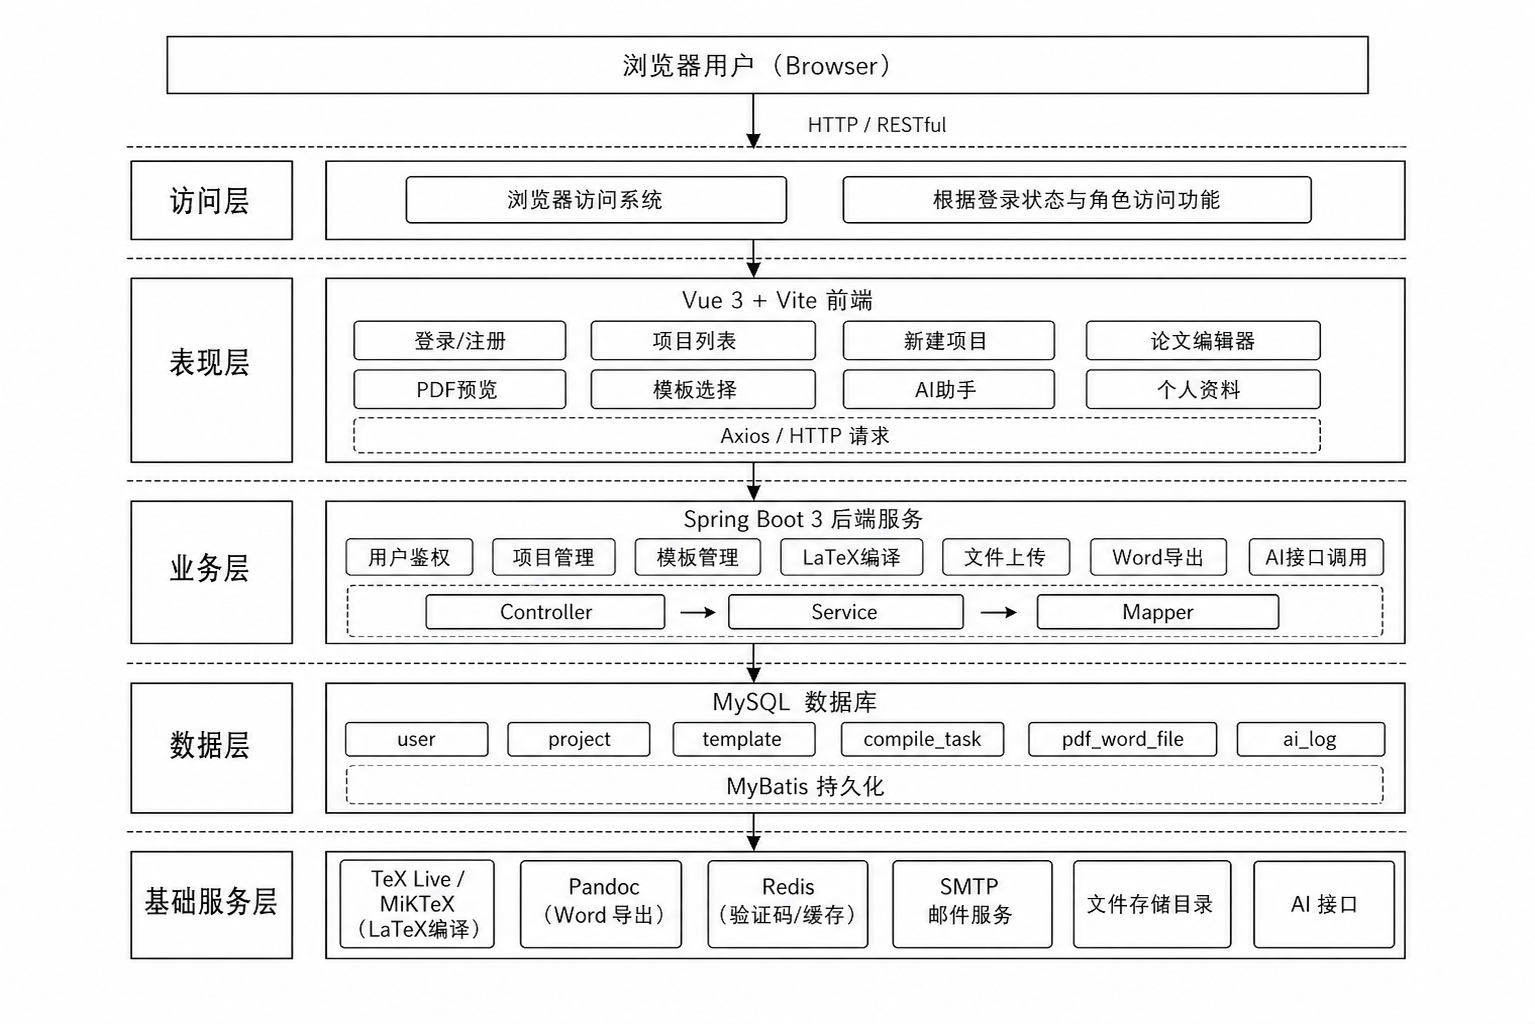
\includegraphics[width=1\linewidth]{project_41_57a8a730.png}
    \caption{系统总体架构图}
    \label{fig:placeholder}
\end{figure}


\section{功能设计}
根据第三章需求分析结果，系统主要划分为用户管理模块、论文项目管理模块、模板管理模块、LaTeX 在线编辑模块、论文编译模块、文件导出模块和 AI 辅助模块。各模块之间既相互独立，又围绕论文项目形成完整业务流程。

（1）用户管理模块。该模块主要负责用户注册、登录、邮箱验证码、个人资料展示和头像上传等功能。用户注册时需要填写邮箱、用户名和密码，系统通过邮箱验证码校验用户邮箱的有效性。用户登录成功后，后端生成 token 并返回给前端，前端在后续请求中携带 token，后端通过拦截器解析 token 获取用户身份。管理员用户在普通用户权限基础上，可以进行模板导入和模板管理操作。

（2）论文项目管理模块。该模块是系统的核心业务模块，主要负责论文项目的创建、查询、修改和删除。用户可以创建空白项目，也可以基于模板创建项目，还可以通过 PDF 导入方式创建项目。项目创建后，系统将项目名称、LaTeX 内容、所属用户和创建时间等信息保存到数据库中。用户进入项目列表页面后，只能查看自己创建的项目，系统通过用户 ID 进行数据隔离。

（3）模板管理模块。该模块用于管理论文模板资源。普通用户可以查看模板列表，并基于模板创建项目。管理员用户可以新增、修改、删除模板，也可以导入完整的 zip 模板包。由于 LaTeX 模板通常包含 .tex、.cls、.sty、.bib、.bst 和图片等依赖文件，因此系统在模板导入时保留模板目录结构，并在编译阶段复制模板依赖目录，保证模板能够正常编译。

（4）LaTeX 在线编辑模块。该模块为用户提供在线论文编辑能力。系统前端集成 CodeMirror 编辑器，用户可以在浏览器中编辑 LaTeX 源码。编辑器页面还提供组件拖拽插入、图片上传、公式插入、编译引擎选择、PDF 预览和 AI 助手等功能。用户修改论文内容后，可以保存到数据库，也可以直接触发编译生成 PDF。

（5）论文编译模块。该模块负责将 LaTeX 源码编译为 PDF 文件。系统支持 pdflatex、xelatex 和 lualatex 三种编译引擎。后端在编译时创建临时目录，处理图片路径和模板依赖文件，然后调用对应编译命令生成 PDF。如果检测到参考文献信息，系统还可以执行 BibTeX 和多轮 LaTeX 编译，以保证引用编号和参考文献结果正确。

（6）文件导出模块。该模块主要负责 PDF、LaTeX 和 Word 文件导出。PDF 文件由 LaTeX 编译生成，LaTeX 文件由项目源码导出，Word 文件通过 Pandoc 等工具转换生成。导出文件信息可以记录到数据库中，便于用户后续下载和系统进行文件管理。

（7）AI 辅助模块。该模块包括 AI 对话辅助、PDF 转 LaTeX 和编译错误分析等功能。用户可以在编辑器页面向 AI 助手提问，获取 LaTeX 语法、论文排版和模板使用方面的帮助。当论文编译失败时，系统可以将编译日志和相关源码片段提交给 AI 接口，由 AI 返回错误原因和修改建议，从而帮助用户提高错误排查效率。

\section{数据库设计}
数据库设计是系统概要设计的重要组成部分。本系统使用 MySQL 数据库存储业务数据，主要包括用户信息、论文项目、模板信息、编译任务、导出文件和 AI 日志等。数据库设计需要保证数据结构清晰、关系明确，并能够满足系统主要业务流程的需要。

\subsection{ER 图}
根据系统业务关系，可以得到以下实体关系：

（1）用户与项目之间是一对多关系。一个用户可以创建多个论文项目，一个论文项目只属于一个用户。

（2）项目与编译任务之间是一对多关系。一个项目可以多次编译，每次编译都会产生一条编译记录。

（3）项目与导出文件之间是一对多关系。一个项目可以导出多个 PDF、Word 或 LaTeX 文件。

（4）项目与 AI 日志之间是一对多关系。一个项目可以产生多次 AI 对话或错误分析记录。

（5）模板与项目之间为逻辑关联关系。用户可以基于模板创建项目，但项目创建后主要保存 LaTeX 内容，不强制依赖模板表外键。

\begin{figure}[!ht]
    \centering
    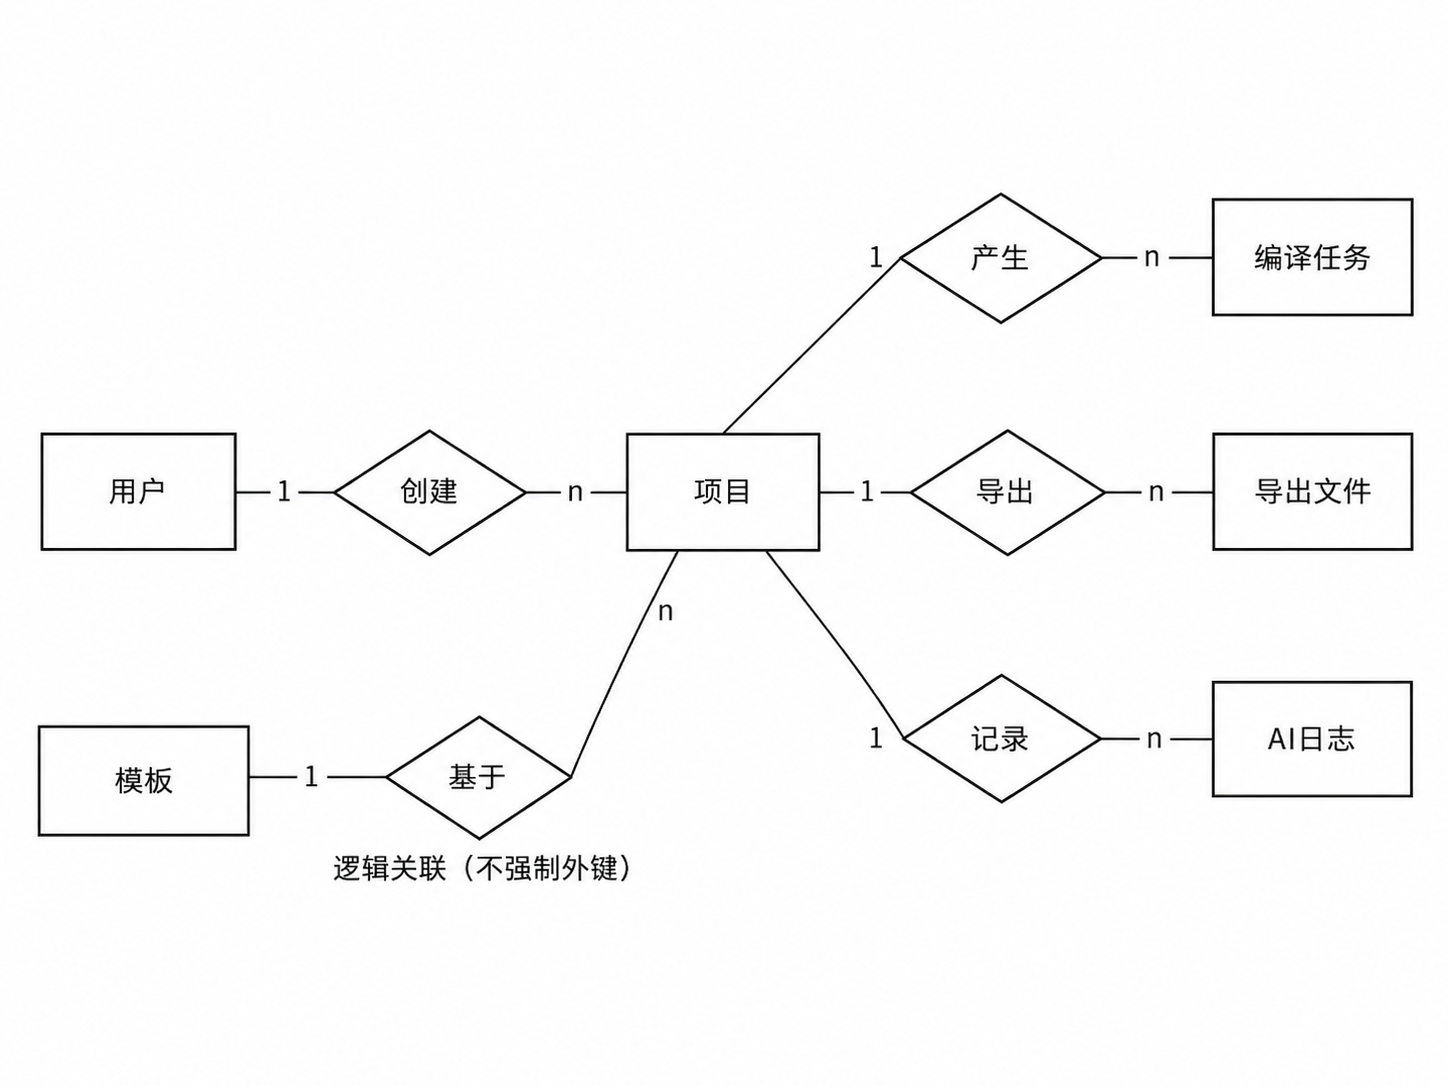
\includegraphics[width=1\linewidth]{project_41_ae365ed8.png}
    \caption{ER 图}
    \label{fig:placeholder}
\end{figure}


\subsection{主要表设计}
本系统主要数据表包括 user、project、template、compile\_task、pdf\_word\_file 和 ai\_log。各表设计如下。 

\begin{table}[!ht]
    \centering
    \caption{用户表 \texttt{user}}
    \label{tab:user}
    \begin{tabular}{|c|c|c|}
        \hline
        \textbf{字段名} & \textbf{类型} & \textbf{说明} \\ \hline
        \texttt{user\_id} & \texttt{bigint} & 用户 ID，主键 \\ \hline
        \texttt{username} & \texttt{varchar} & 用户名 \\ \hline
        \texttt{email} & \texttt{varchar} & 邮箱 \\ \hline
        \texttt{password\_hash} & \texttt{varchar} & 密码哈希 \\ \hline
        \texttt{avatar\_url} & \texttt{varchar} & 头像地址 \\ \hline
        \texttt{role} & \texttt{varchar} & 用户角色 \\ \hline
    \end{tabular}
\end{table}

用户表用于保存系统用户基本信息。其中 password\_hash 字段用于保存加密后的密码，role 字段用于区分普通用户和管理员。

\begin{table}[!ht]
    \centering
    \caption{项目表 \texttt{project}}
    \label{tab:project}
    \begin{tabular}{|c|c|c|}
        \hline
        \textbf{字段名} & \textbf{类型} & \textbf{说明} \\ \hline
        \texttt{project\_id} & \texttt{bigint} & 项目 ID，主键 \\ \hline
        \texttt{name} & \texttt{varchar} & 项目名称 \\ \hline
        \texttt{latex\_content} & \texttt{text} & LaTeX 源码内容 \\ \hline
        \texttt{user\_id} & \texttt{bigint} & 所属用户 ID \\ \hline
        \texttt{created\_at} & \texttt{datetime} & 创建时间 \\ \hline
        \texttt{updated\_at} & \texttt{datetime} & 更新时间 \\ \hline
    \end{tabular}
\end{table}

项目表是系统核心业务表，用于保存用户论文项目内容。论文编辑、编译、导出等功能均以 project 表中的 LaTeX 内容为基础。

\begin{table}[!ht]
    \centering
    \caption{模板表 \texttt{template}}
    \label{tab:template}
    \begin{tabular}{|c|c|c|}
        \hline
        \textbf{字段名} & \textbf{类型} & \textbf{说明} \\ \hline
        \texttt{template\_id} & \texttt{bigint} & 模板 ID，主键 \\ \hline
        \texttt{name} & \texttt{varchar} & 模板名称 \\ \hline
        \texttt{description} & \texttt{varchar} & 模板描述 \\ \hline
        \texttt{template\_path} & \texttt{varchar} & 模板文件路径 \\ \hline
        \texttt{preview\_url} & \texttt{varchar} & 模板预览地址 \\ \hline
        \texttt{created\_at} & \texttt{datetime} & 创建时间 \\ \hline
    \end{tabular}
\end{table}

模板表用于保存论文模板信息。管理员导入 zip 模板包后，系统将模板文件保存到服务器目录，并将模板路径记录到数据库中。

\begin{table}[!ht]
    \centering
    \caption{编译任务表 \texttt{compile\_task}}
    \label{tab:compile-task}
    \begin{tabular}{|c|c|c|}
        \hline
        \textbf{字段名} & \textbf{类型} & \textbf{说明} \\ \hline
        \texttt{task\_id} & \texttt{bigint} & 编译任务 ID \\ \hline
        \texttt{project\_id} & \texttt{bigint} & 项目 ID \\ \hline
        \texttt{engine} & \texttt{varchar} & 编译引擎 \\ \hline
        \texttt{status} & \texttt{varchar} & 编译状态 \\ \hline
        \texttt{log} & \texttt{text} & 编译日志 \\ \hline
        \texttt{result\_pdf\_path} & \texttt{varchar} & PDF 文件路径 \\ \hline
        \texttt{created\_at} & \texttt{datetime} & 创建时间 \\ \hline
        \texttt{completed\_at} & \texttt{datetime} & 完成时间 \\ \hline
    \end{tabular}
\end{table}

编译任务表用于记录项目每次编译结果。系统可以通过该表查询最近一次编译状态，并在编译失败时获取错误日志。

\begin{table}[!ht]
    \centering
    \caption{导出文件表 \texttt{pdf\_word\_file}}
    \label{tab:pdf-word-file}
    \begin{tabular}{|c|c|c|}
        \hline
        \textbf{字段名} & \textbf{类型} & \textbf{说明} \\ \hline
        \texttt{pdf\_id} & \texttt{bigint} & 文件记录 ID \\ \hline
        \texttt{project\_id} & \texttt{bigint} & 项目 ID \\ \hline
        \texttt{filename} & \texttt{varchar} & 文件名称 \\ \hline
        \texttt{file\_path} & \texttt{varchar} & 文件路径 \\ \hline
        \texttt{uploaded\_at} & \texttt{datetime} & 创建时间 \\ \hline
    \end{tabular}
\end{table}

该表用于记录系统生成的 PDF、Word 等导出文件，便于用户下载和系统管理历史文件。

\begin{table}[!ht]
    \centering
    \caption{AI 日志表 \texttt{ai\_log}}
    \label{tab:ai-log}
    \begin{tabular}{|c|c|c|}
        \hline
        \textbf{字段名} & \textbf{类型} & \textbf{说明} \\ \hline
        \texttt{id} & \texttt{bigint} & 日志 ID \\ \hline
        \texttt{project\_id} & \texttt{bigint} & 项目 ID \\ \hline
        \texttt{request\_type} & \texttt{varchar} & 请求类型 \\ \hline
        \texttt{input\_content} & \texttt{text} & 输入内容 \\ \hline
        \texttt{output\_content} & \texttt{text} & 输出内容 \\ \hline
        \texttt{created\_at} & \texttt{datetime} & 创建时间 \\ \hline
    \end{tabular}
\end{table}

AI 日志表用于记录 AI 对话和编译错误分析过程，便于后续问题追踪和功能优化。

\section{界面设计}
界面设计直接影响用户使用体验。本系统主要面向不一定熟悉 LaTeX 的普通用户，因此界面设计应尽量简洁、清晰，使用户能够快速完成论文创建、编辑、编译和导出操作。系统主要界面包括登录注册页面、项目列表页面、新建项目页面、编辑器页面和个人资料页面。

\subsection{登录注册页面设计}
登录注册页面是用户进入系统的入口。登录页面主要包括账号输入框、密码输入框和登录按钮。注册页面主要包括用户名、邮箱、密码、验证码输入框和发送验证码按钮。用户完成注册后可以使用账号登录系统。登录成功后，系统跳转至项目列表页面。

\begin{figure}[!ht]
    \centering
    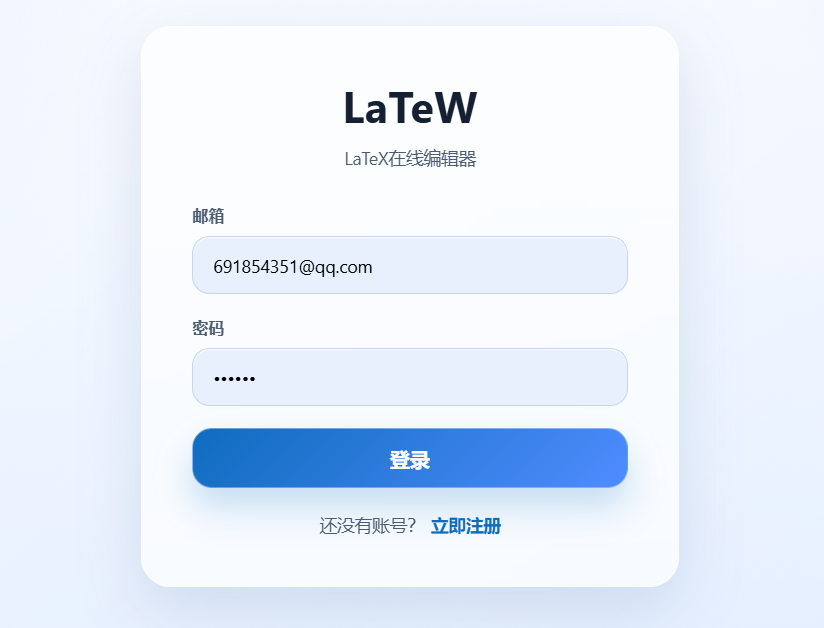
\includegraphics[width=1\linewidth]{project_41_a472e2ed.png}
    \caption{登录注册页面设计}
    \label{fig:placeholder}
\end{figure}

\subsection{项目列表与新建项目页面设计}

项目列表页面用于展示当前用户已有论文项目。页面应显示项目名称、更新时间和操作按钮，用户可以进入编辑、删除项目或下载编译结果。管理员用户在该页面可以看到模板导入入口。

\begin{figure}[!ht]
    \centering
    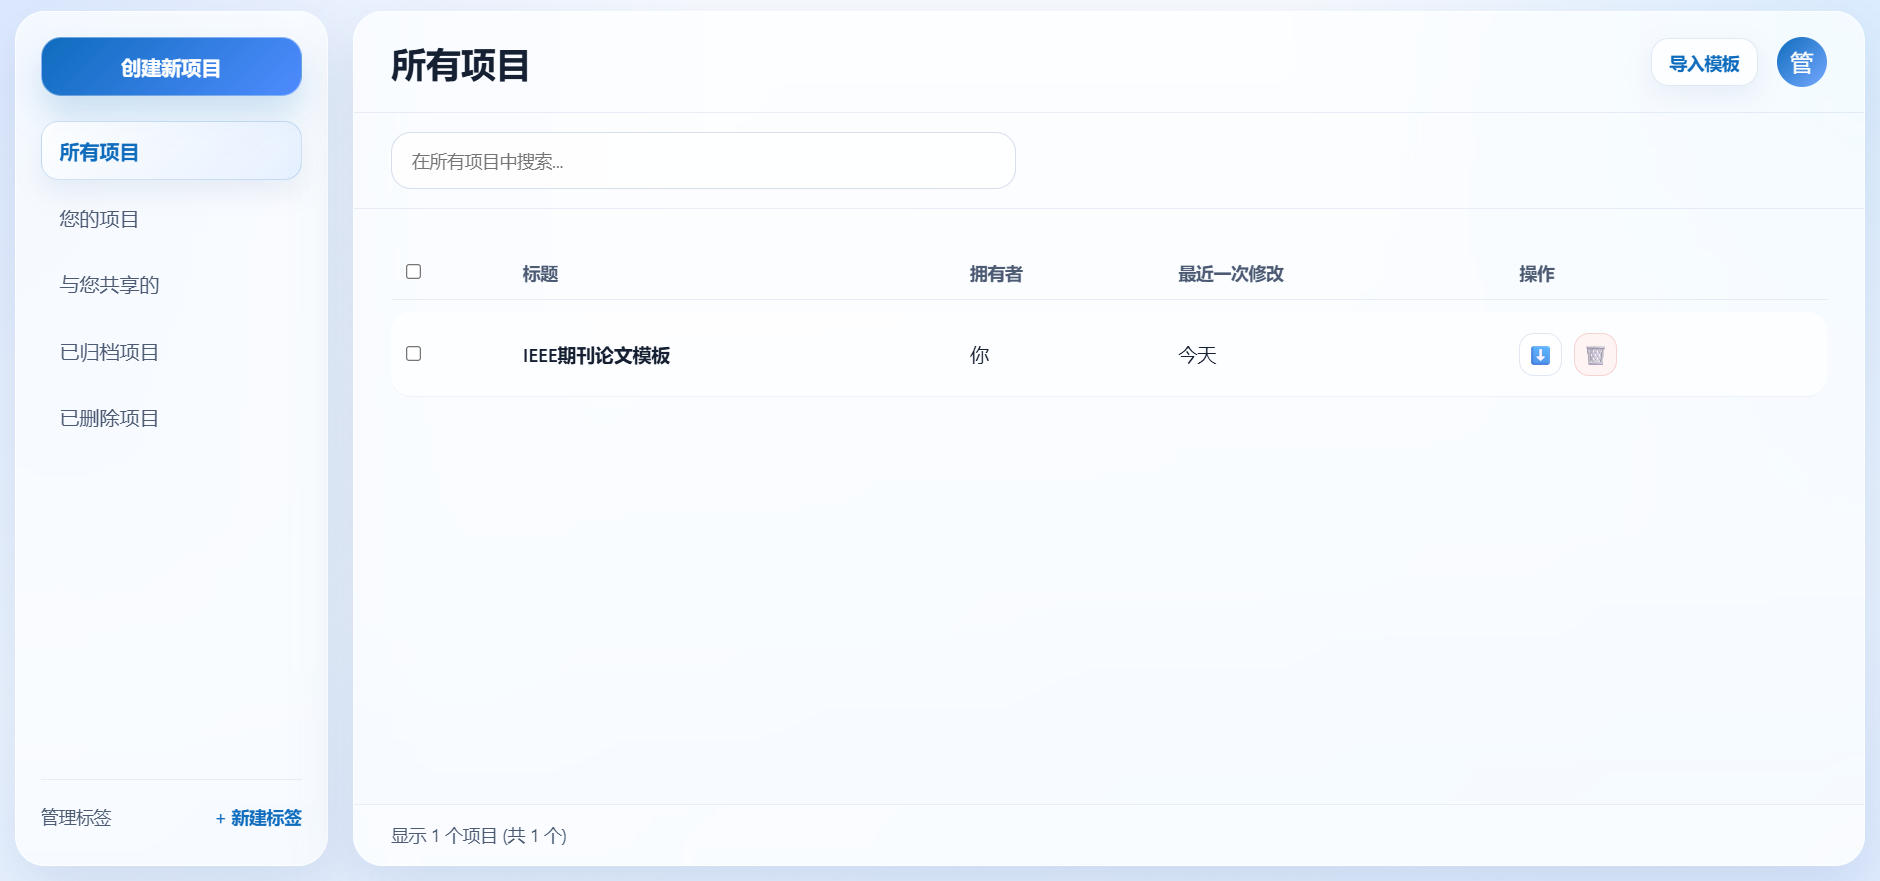
\includegraphics[width=1\linewidth]{project_41_01b6e725.png}
    \caption{项目列表页面设计}
    \label{fig:placeholder}
\end{figure}

新建项目页面提供三种创建方式：空白创建、模板创建和 PDF 导入创建。空白创建适合用户自行编写论文；模板创建适合用户快速生成论文基本结构；PDF 导入创建则适合用户将已有 PDF 内容转换为 LaTeX 项目。

\begin{figure}[!ht]
    \centering
    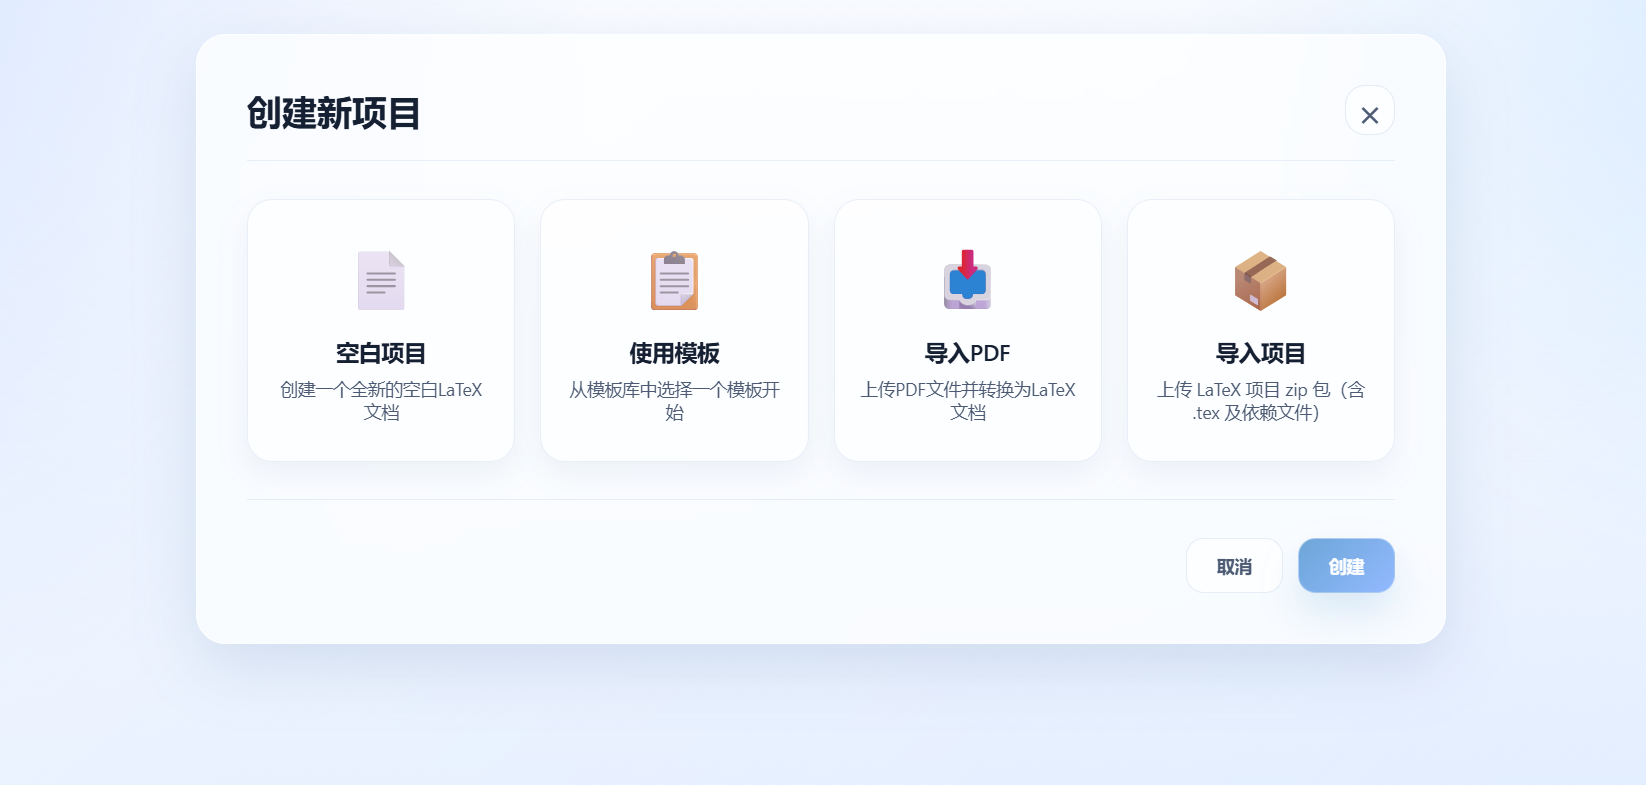
\includegraphics[width=1\linewidth]{project_41_0db2a899.png}
    \caption{新建项目页面设计}
    \label{fig:placeholder}
\end{figure}

\subsection{编辑器页面设计}
编辑器页面是系统最核心的页面。该页面主要分为三个区域：左侧或上方为工具栏，中间为 LaTeX 源码编辑区，右侧为 PDF 预览区。工具栏提供导入tex文件、保存、编译、选择编译引擎、导出 PDF、导出 Word、导出 LaTeX 等操作。源码编辑区用于编辑 LaTeX 内容，PDF 预览区用于展示编译结果和错误日志。

在编辑器页面中，用户可以完成从论文编辑到编译预览的主要流程。当编译成功时，系统刷新 PDF 预览区域；当编译失败时，系统显示错误日志，并提供 AI 分析入口。这样的界面设计可以减少页面跳转，使论文写作流程更加连贯。

\begin{figure}[!ht]
    \centering
    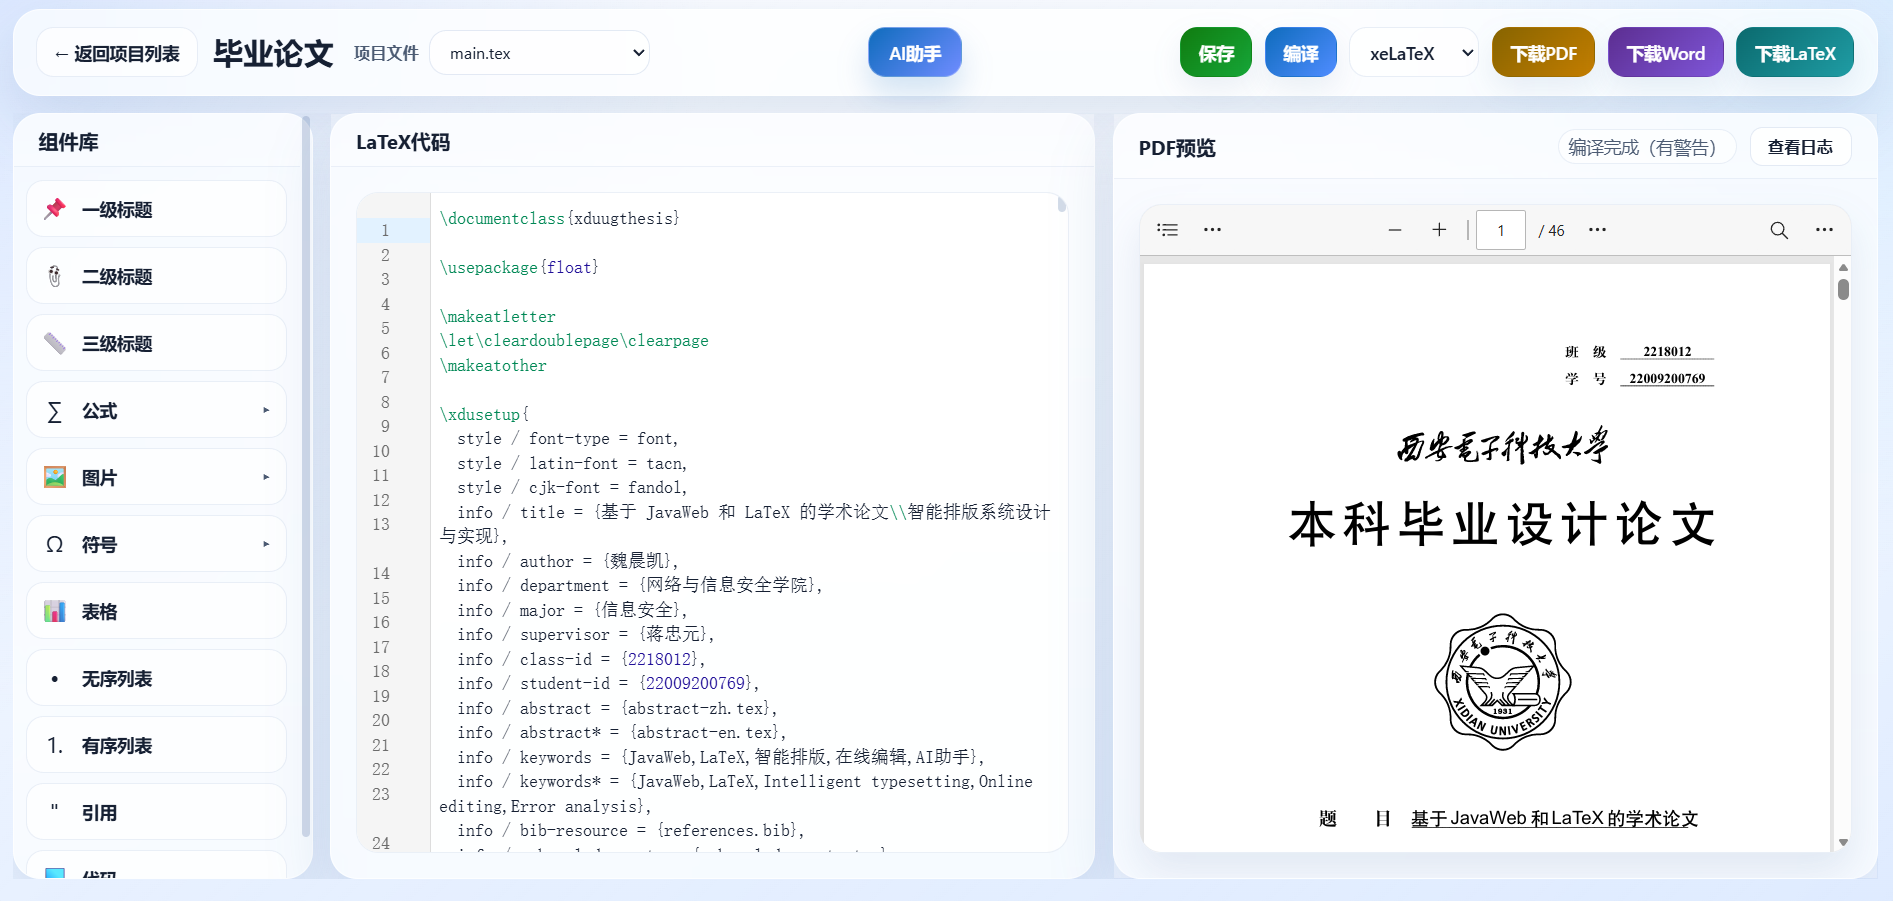
\includegraphics[width=1\linewidth]{project_41_3acb8d2d.png}
    \caption{编辑器页面设计}
    \label{fig:placeholder}
\end{figure}

\subsection{个人资料页面设计}
个人资料页面用于展示和修改用户基本信息。页面主要包括头像、用户名、邮箱和用户ID。用户可以上传头像或修改用户名。该页面作为用户管理模块的补充，增强系统的完整性。

\begin{figure}[!ht]
    \centering
    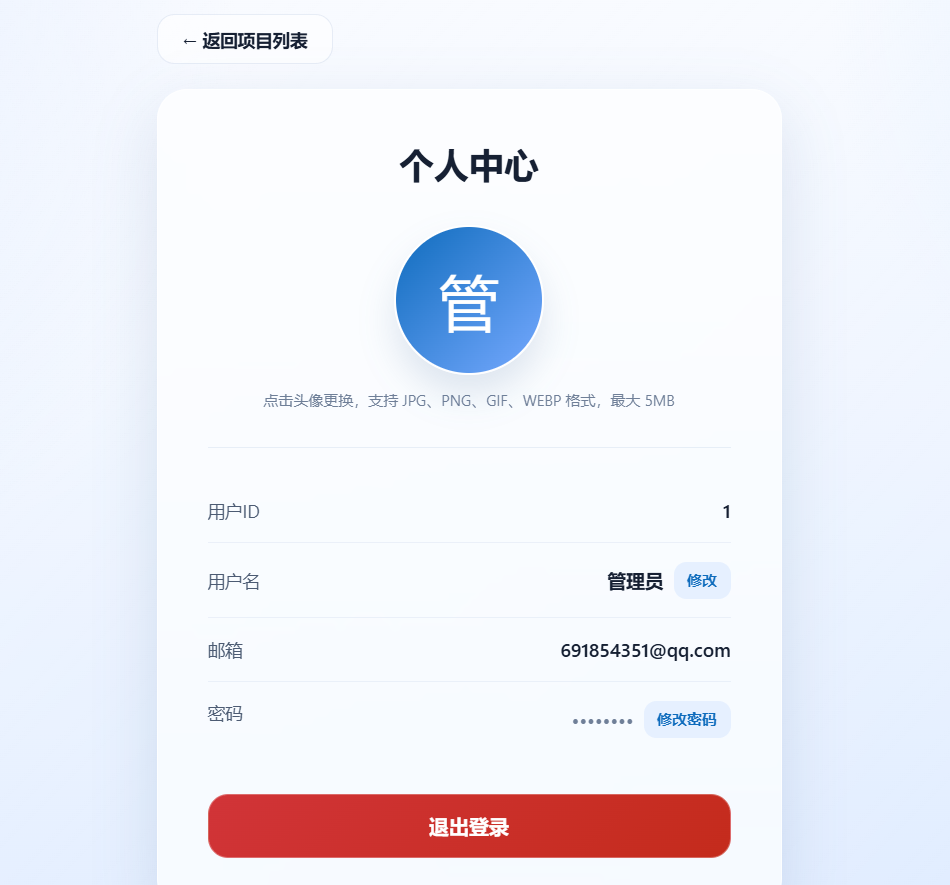
\includegraphics[width=1\linewidth]{project_41_ad21c55b.png}
    \caption{个人资料页面设计}
    \label{fig:placeholder}
\end{figure}

\section{本章小结}
本章对基于 JavaWeb 和 LaTeX 的学术论文智能排版系统进行了概要设计。首先介绍了系统总体架构，明确系统采用 B/S 架构和前后端分离模式，并从访问层、表现层、业务层、数据层和基础服务层对系统结构进行了划分。其次，根据需求分析结果，对系统功能模块进行了设计，包括用户管理、论文项目管理、模板管理、LaTeX 在线编辑、论文编译、文件导出和 AI 辅助等模块。然后，对系统数据库进行了概要设计，说明了主要实体关系和核心数据表结构。最后，对系统主要界面进行了设计，包括登录注册页面、项目列表页面、新建项目页面、编辑器页面和个人资料页面。本章内容为下一章系统详细设计与实现提供了基础。

\chapter{系统详细设计与实现}
本章在前文需求分析和概要设计的基础上，对基于 JavaWeb 和 LaTeX 的学术论文智能排版系统进行详细设计与实现说明。系统采用前后端分离架构，前端主要负责用户界面展示和交互操作，后端主要负责业务逻辑处理、数据库访问、文件管理、LaTeX 编译和 AI 接口调用。本章将从开发环境、系统框架、用户管理、论文项目管理、模板管理、LaTeX 在线编辑、论文编译与预览、AI 辅助等方面展开说明。

与普通在线编辑系统不同，本文系统的实现重点不只是完成 LaTeX 源码编辑和 PDF 编译，而是围绕本科毕业论文写作过程中常见的实际问题进行功能设计。传统 LaTeX 写作方式虽然排版能力较强，但用户需要记忆较多 LaTeX 命令，并且需要自行处理模板文件、编译环境和编译错误等问题。针对这些问题，系统在编辑器中加入组件拖入、模板载入、在线编译预览和辅助分析等功能，使用户能够在浏览器中完成论文写作与排版操作。

\section{开发环境}

本系统开发过程中使用的主要软硬件环境如表5.1所示。

\begin{table}[!ht]
    \centering
    \caption{系统开发环境}
    \label{tab:development-environment}
    \begin{tabular}{|c|c|}
        \hline
        \textbf{环境类型} & \textbf{配置内容} \\ \hline
        操作系统 & Windows 11 \\ \hline
        前端框架 & Vue 3、Vite \\ \hline
        前端编辑器 & Visual Studio Code \\ \hline
        后端框架 & Spring Boot 3 \\ \hline
        后端语言 & Java \\ \hline
        持久层框架 & MyBatis \\ \hline
        数据库 & MySQL \\ \hline
        缓存服务 & Redis \\ \hline
        \LaTeX{} 编译环境 & TeX Live \\ \hline
        文档转换工具 & Pandoc \\ \hline
        主要开发工具 & IntelliJ IDEA、DataGrip、Cursor \\ \hline
        浏览器 & Chrome / Edge \\ \hline
    \end{tabular}
\end{table}

系统前端采用 Vue 3 和 Vite 进行开发，利用组件化方式组织页面结构。后端采用 Spring Boot 3 构建 RESTful 接口，使用 MyBatis 完成数据库访问。数据库采用 MySQL 保存用户、项目、模板、编译任务和 AI 日志等信息。LaTeX 编译功能依赖 TeX Live 环境，Word 导出功能依赖 Pandoc 等文档转换工具。

\section{用户管理模块的设计与实现}
用户管理模块主要实现用户注册、登录、邮箱验证码、个人资料和头像上传等功能。该模块是系统的基础模块，后续项目管理、模板管理、论文编译和 AI 辅助等功能都依赖用户身份信息。

用户注册流程为：用户在注册页面填写用户名、邮箱、密码和验证码，前端提交注册请求，后端首先校验邮箱验证码是否正确，然后判断邮箱或用户名是否已存在。如果校验通过，后端对密码进行加密处理，并将用户信息保存到 user 表中。

用户登录流程为：用户输入账号和密码后，后端根据账号查询用户信息，并对用户输入密码与数据库中保存的加密密码进行匹配。验证通过后，系统生成 token 返回给前端。前端保存 token 后，用户即可访问项目列表、编辑器等页面。

用户管理模块的实现重点如下：

（1）密码加密存储。

系统不直接保存用户明文密码，而是在后端对密码进行加密后存储。这样即使数据库信息泄露，也可以降低用户密码被直接获取的风险。

（2）邮箱验证码校验。

系统通过邮件服务向用户邮箱发送验证码，并将验证码临时保存到 Redis 中，同时设置有效时间。用户注册时，后端校验验证码是否正确和是否过期。

（3）登录状态验证。

用户登录成功后，系统生成 token。后续请求中，前端需要在请求头中携带 token，后端通过拦截器解析 token，获取当前用户 ID，并完成权限校验。

（4）头像上传。

用户可以上传头像文件，后端接收文件后保存到服务器指定目录，并将头像访问路径写入用户表。

\begin{figure}[!ht]
    \centering
    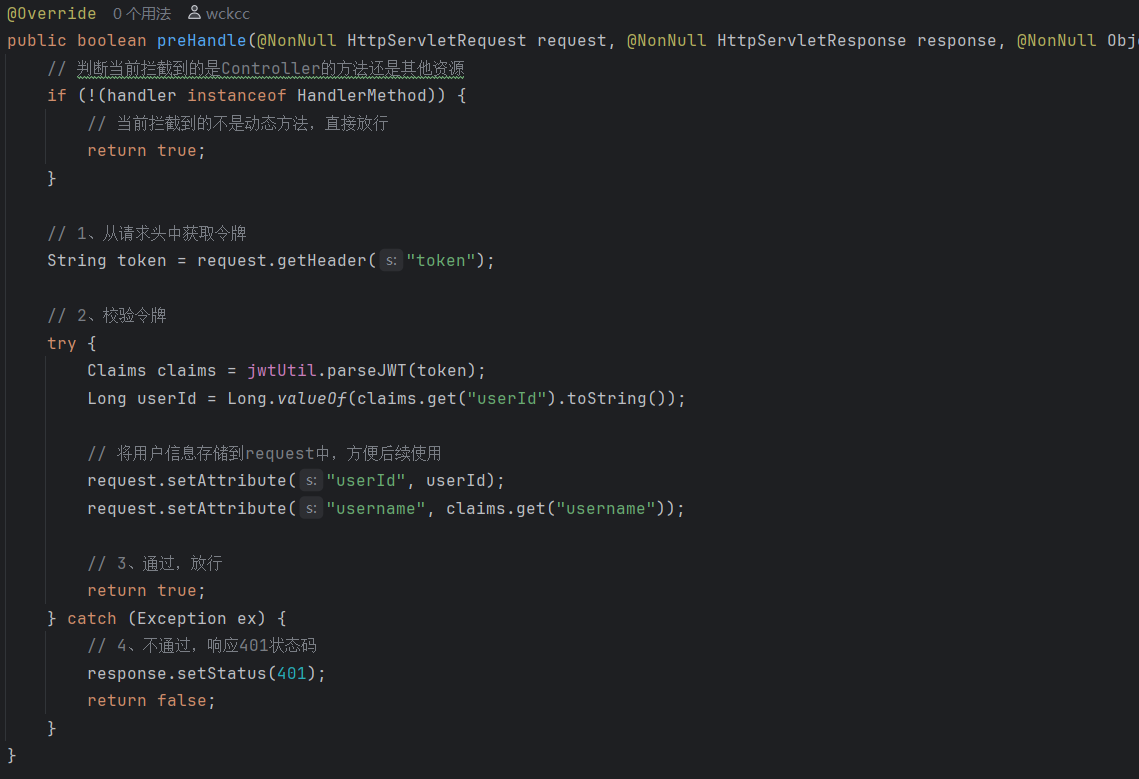
\includegraphics[width=0.75\linewidth]{project_41_832e9124.png}
    \caption{登录校验代码片段}
    \label{fig:placeholder}
\end{figure}

\section{论文项目管理模块的设计与实现}
论文项目管理模块是系统的核心模块，用户所有论文内容都以项目为单位进行保存和管理。系统支持空白项目创建、模板项目创建、PDF 导入项目、项目列表查询、项目编辑保存和项目删除等功能。

项目创建时，用户可以选择不同方式。如果用户创建空白项目，系统会生成一个基础 LaTeX 文档结构；如果用户基于模板创建项目，系统会读取模板内容并写入新项目；如果用户通过 PDF 导入创建项目，系统会调用相关解析或 AI 服务，将 PDF 内容转换为 LaTeX 初始内容。

项目保存时，前端将编辑器中的 LaTeX 源码提交给后端，后端根据项目 ID 和当前用户 ID 查询项目是否存在，并判断项目是否属于当前用户。校验通过后，后端更新 project 表中的 latex\_content 和 updated\_at 字段。

项目删除时，系统同样需要进行权限校验，防止用户删除他人的项目。删除操作可以采用物理删除，也可以采用逻辑删除方式。本系统是直接删除项目记录，但在后续扩展中可以增加回收站功能。

\begin{figure}[!ht]
    \centering
    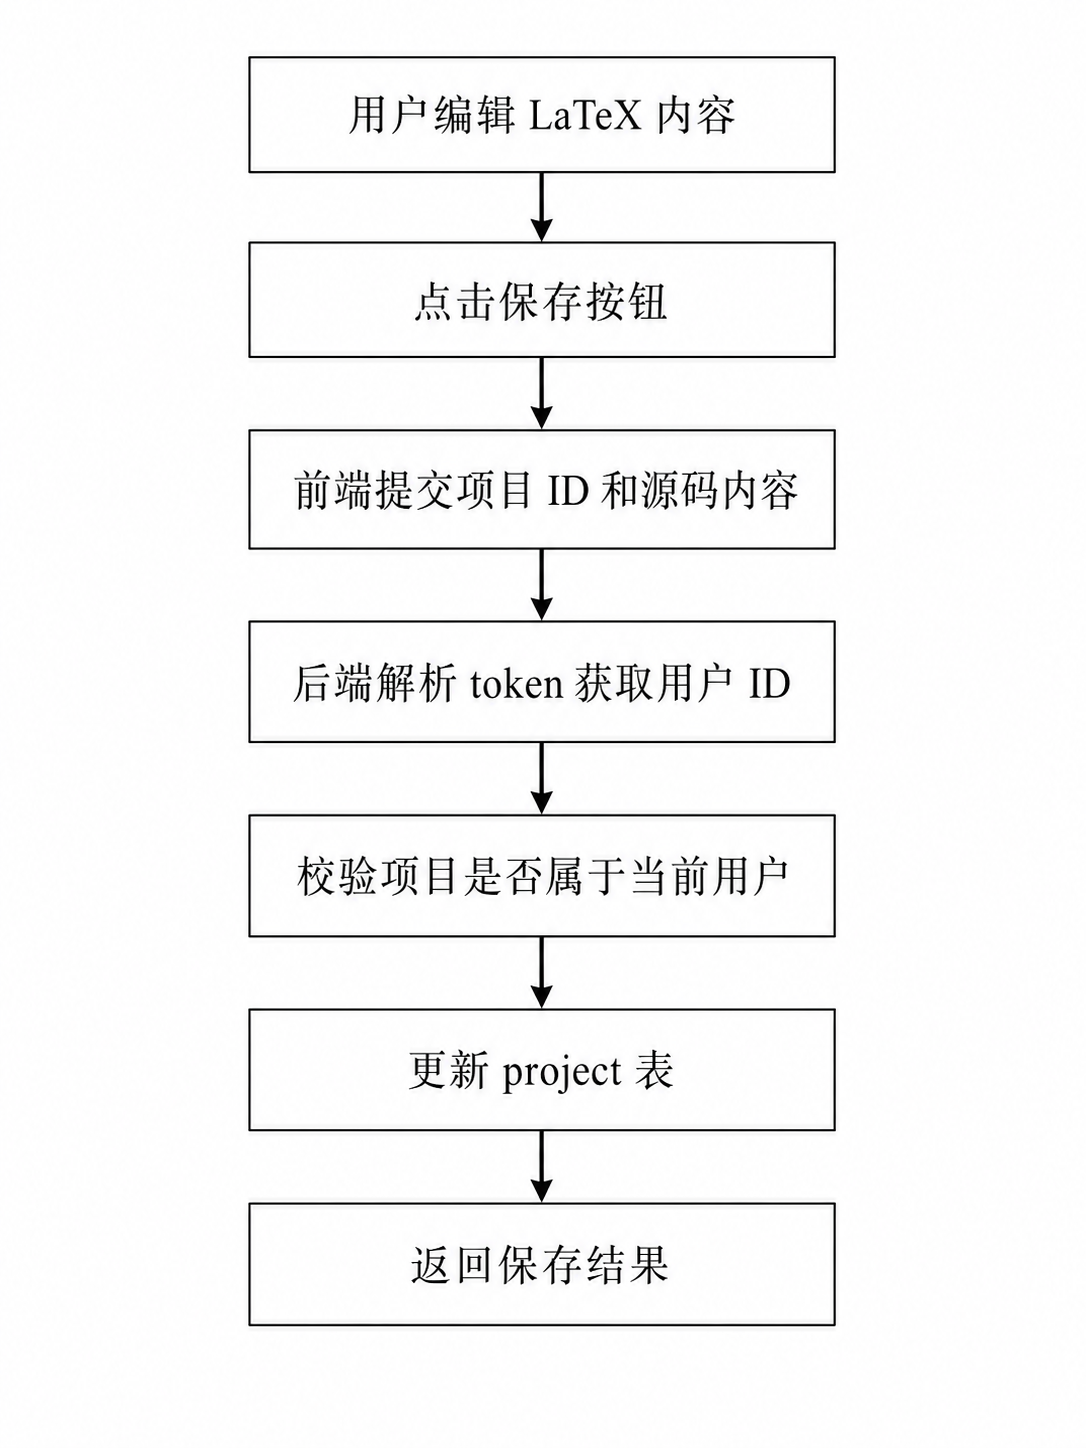
\includegraphics[width=0.75\linewidth]{project_41_ba93d89d.png}
    \caption{项目保存流程图}
    \label{fig:placeholder}
\end{figure}

\begin{figure}[!ht]
    \centering
    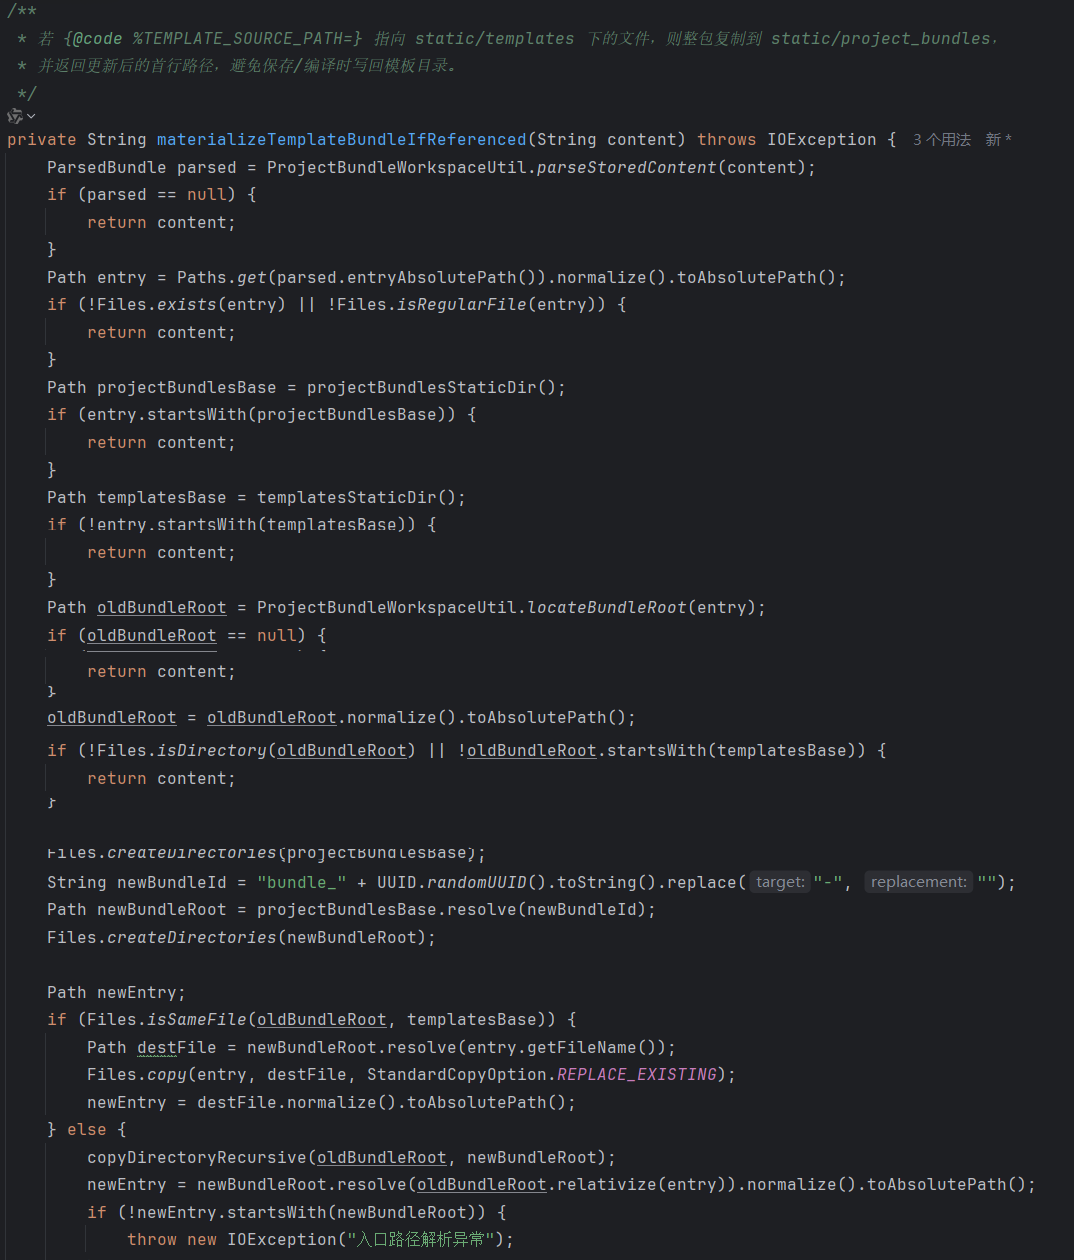
\includegraphics[width=0.75\linewidth]{project_41_f5cf93be.png}
    \caption{更新项目代码片段}
    \label{fig:placeholder}
\end{figure}

\section{模板管理模块的设计与实现}
模板管理模块用于帮助用户快速创建符合格式要求的论文项目。系统模板主要包括模板名称、模板描述、模板文件路径等。普通用户可以查看模板列表并基于模板创建项目，管理员可以新增模板，并上传完整的 zip 模板包。

LaTeX 模板通常不只是一个 .tex 文件，还可能包含 .cls、.sty、.bib、.bst、图片和字体配置等依赖资源。如果系统只保存主 tex 文件，编译时容易出现样式缺失或依赖文件找不到的问题。因此，本系统在模板导入时采用完整 zip 包导入方式，后端解压模板包后保留原始目录结构，并记录模板主文件路径。

模板导入流程为：管理员上传 zip 文件，后端首先校验文件类型，然后解压到模板存储目录。解压完成后，系统扫描目录中的 tex 文件，并选择主 tex 文件作为模板入口。管理员填写模板名称和描述后，系统将模板信息保存到 template 表中。用户基于模板创建项目时，系统读取模板主文件内容，并复制模板依赖目录到项目编译目录中。

模板导入设计的关键在于保留依赖文件。系统在编译基于模板创建的项目时，需要将模板目录中的依赖文件复制到临时编译目录，使 LaTeX 编译器能够找到对应的样式文件、参考文献文件和图片资源。

\begin{figure}[!ht]
    \centering
    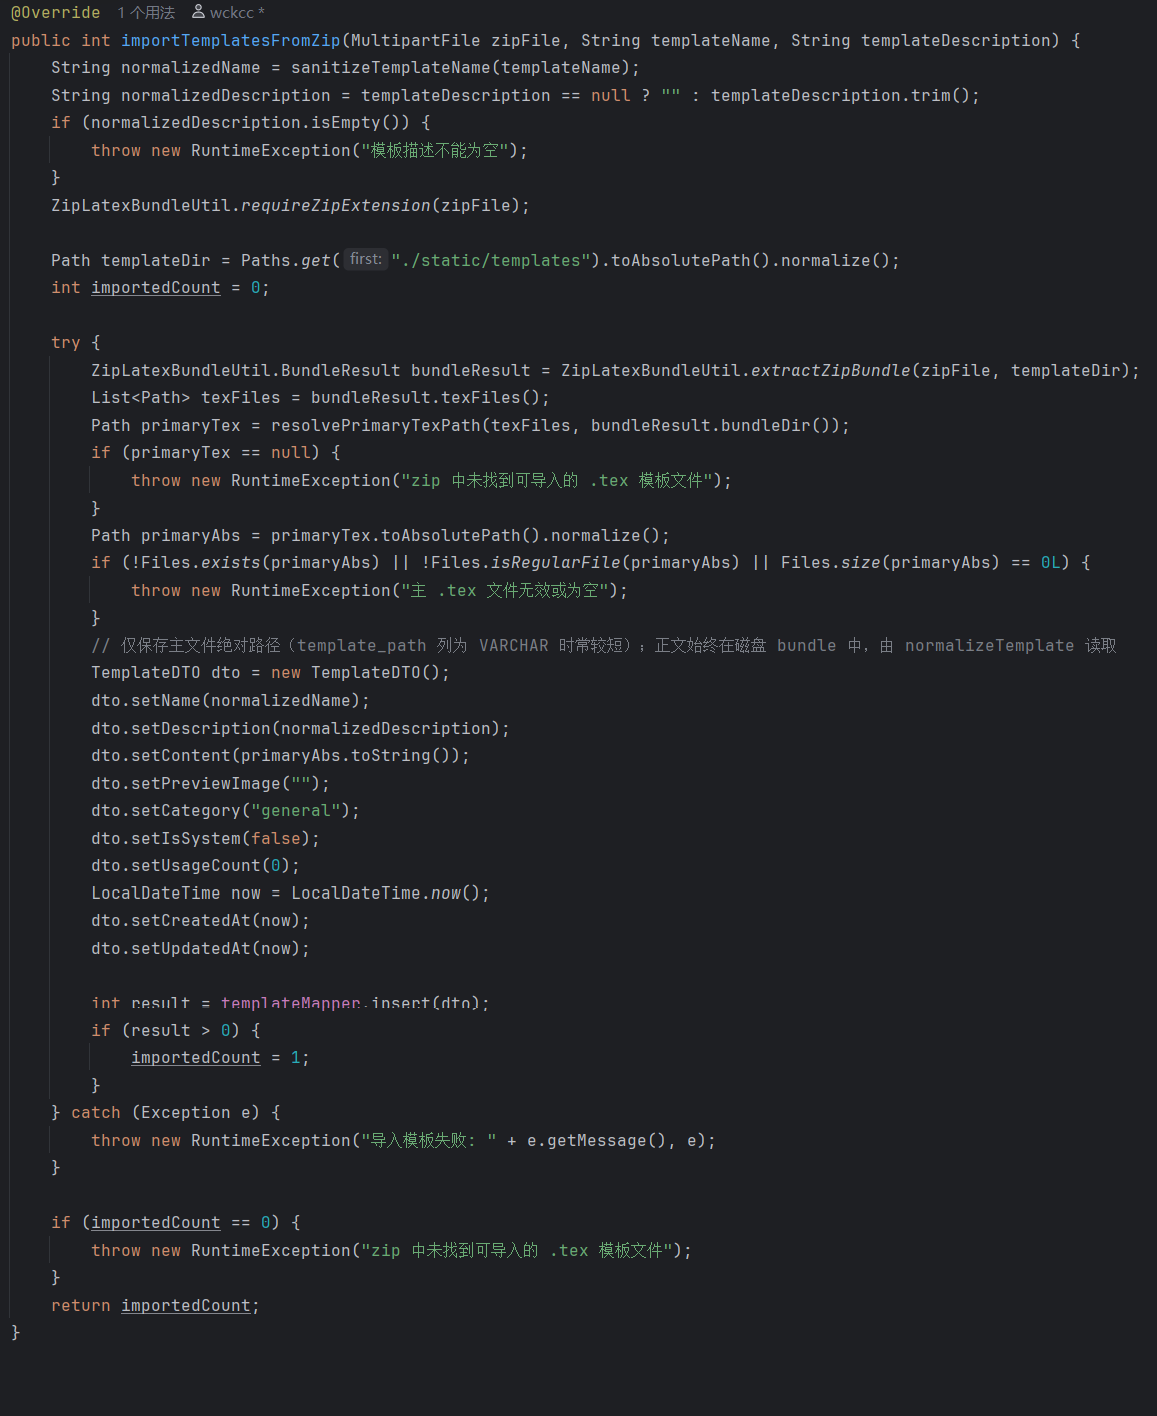
\includegraphics[width=0.75\linewidth]{project_41_77d9206c.png}
    \caption{模板导入代码片段}
    \label{fig:placeholder}
\end{figure}

传统 LaTeX 使用方式下，用户需要先下载模板压缩包，然后在本地手动解压，查找主 tex 文件，并确认 cls、sty、bib、bst、图片等依赖文件是否完整。如果用户只复制了主 tex 文件，而没有保留其他依赖文件，编译时就可能出现找不到样式文件、参考文献样式缺失或图片无法显示等问题。

在本系统中，管理员可以直接上传完整 zip 模板包，系统解压后保留模板目录结构。用户创建论文项目时，只需要在模板列表中选择对应模板，系统即可将模板内容载入编辑器，并在后续编译时复制模板依赖文件。这样可以减少用户手动处理模板文件的过程，使模板使用更加直观。

\begin{table}[!ht]
    \centering
    \caption{模板导入案例运行过程}
    \label{tab:template-import-case}
    \begin{tabular}{|c|p{5cm}|p{6cm}|}
        \hline
        步骤 & 操作内容 & 运行结果 \\
        \hline
        1 & 管理员上传完整 zip 模板包 & 系统校验文件类型并完成模板解压 \\
        \hline
        2 & 系统扫描模板目录 & 识别主 tex 文件，并保留 cls、sty、bib 等依赖文件 \\
        \hline
        3 & 用户选择模板创建项目 & 编辑器中成功载入模板初始内容 \\
        \hline
        4 & 用户修改论文题目和章节内容 & 修改后的 LaTeX 内容能够正常保存 \\
        \hline
        5 & 用户编译模板项目 & 系统复制模板依赖并生成 PDF 预览结果 \\
        \hline
    \end{tabular}
\end{table}

模板导入功能与传统模板使用方式的对比如表 \ref{tab:template-compare} 所示。

\begin{table}[!ht]
    \centering
    \caption{模板导入功能与传统模板使用方式对比}
    \label{tab:template-compare}
    \begin{tabular}{|c|p{5cm}|p{5cm}|}
        \hline
        对比项 & 传统 LaTeX 模板使用方式 & 本系统模板使用方式 \\
        \hline
        模板获取 & 用户自行下载并解压模板文件 & 管理员统一导入模板包 \\
        \hline
        主文件判断 & 用户需要自行判断主 tex 文件 & 系统扫描并记录模板主文件 \\
        \hline
        依赖文件处理 & 用户需要手动保留 cls、sty、bib 等文件 & 系统保留模板目录结构 \\
        \hline
        模板复用 & 每次使用都需要重新整理模板文件 & 用户可直接从模板列表创建项目 \\
        \hline
        使用难度 & 对 LaTeX 初学者不够友好 & 操作过程更接近普通 Web 系统 \\
        \hline
    \end{tabular}
\end{table}

通过该案例可以看出，模板管理模块解决了传统 LaTeX 模板使用中“文件多、依赖多、主文件不易判断”的问题。对于本科毕业论文写作场景而言，用户更关心如何快速生成符合格式要求的论文项目，而不是模板底层文件之间的依赖关系。因此，系统通过模板统一导入和模板列表创建项目的方式，降低了用户直接使用 LaTeX 模板的难度。

\section{LaTeX 在线编辑模块的设计与实现}
LaTeX 在线编辑模块为用户提供浏览器端论文源码编辑功能。系统前端集成 CodeMirror 编辑器，使用户能够获得较好的代码编辑体验。编辑器页面主要包括源码编辑区、PDF 预览区和工具栏区域。

源码编辑区用于显示和修改 LaTeX 内容。用户进入编辑页面后，前端根据项目 ID 请求后端项目详情接口，后端返回项目名称和 LaTeX 内容，前端将内容加载到编辑器中。用户修改内容后，可以点击保存按钮，将当前源码保存到数据库。

工具栏主要提供导入tex文件、保存、编译、导出、AI助手、图片上传、公式插入等操作。用户点击图片上传后，前端提交图片文件给后端，后端保存图片并返回访问路径，前端自动生成 LaTeX 图片插入代码。公式插入功能则通过预设常用公式模板实现。用户选择某个公式后，前端将对应 LaTeX 公式代码插入到光标位置，减少用户手动输入复杂命令的成本。

除普通源码编辑外，本系统在编辑器页面中设计了组件拖入功能。页面左侧提供常用论文组件，例如章节、图片、表格、公式、列表、参考文献等。用户可以将组件拖入编辑区域，系统根据组件类型自动生成对应的 LaTeX 代码框架，并插入到编辑器当前光标位置。该功能的核心目标是减少用户对 LaTeX 结构代码的记忆负担。

组件拖入功能的实现流程如下：

（1）前端定义组件列表。系统将常用 LaTeX 结构封装为组件对象，每个组件包含名称、类型、说明和对应的 LaTeX 模板代码。

（2）用户拖动组件。用户在组件栏中选择需要的组件，例如图片、表格或公式，并将其拖动到编辑器区域。

（3）识别组件类型。前端监听拖拽事件，获取被拖动组件的类型和模板内容。

（4）生成代码片段。系统根据组件类型生成对应 LaTeX 代码，例如图片组件生成 figure 环境，表格组件生成 table 和 tabular 环境。

（5）插入编辑器。前端调用 CodeMirror 的插入方法，将生成的代码插入到当前光标位置。

\begin{figure}[!ht]
    \centering
    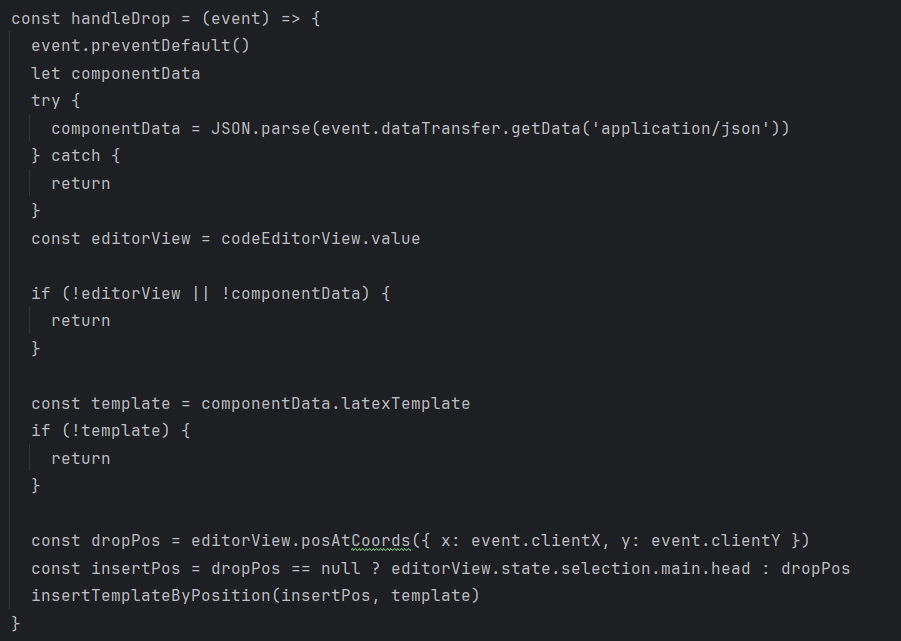
\includegraphics[width=0.75\linewidth]{project_41_b9a69bf1.png}
    \caption{拖拽插入代码片段}
    \label{fig:placeholder}
\end{figure}

传统 LaTeX 写作过程中，用户需要掌握较多命令和环境结构。例如，在论文中插入图片时，用户不仅需要知道图片环境的基本写法，还需要设置图片路径、图片标题和引用标签；插入表格时，需要了解表格环境、列格式、横线和单元格排列方式；插入公式时，也需要掌握公式环境和常用数学符号的写法。对于 LaTeX 初学者而言，这些内容虽然能够实现较好的排版效果，但学习成本较高，在实际编写过程中容易出现环境未闭合、命令拼写错误、括号缺失和参数设置不当等问题。

针对上述问题，本系统在 LaTeX 在线编辑模块中设计了组件拖入功能。用户在写作过程中，不需要从头记忆和输入完整的 LaTeX 结构代码，只需要在组件栏中选择所需组件，并将其拖入编辑区域，系统即可在当前光标位置自动生成对应的代码框架。用户随后只需要根据论文内容修改标题、图片路径、表格内容或公式内容，即可完成相应结构的插入。

以插入图片为例，传统方式下用户需要手动编写完整的图片结构，包括图片环境、居中设置、图片路径、图片标题和标签等内容。如果用户遗漏图片环境的结束语句，或者将图片插入命令拼写错误，就可能导致编译失败。使用本系统时，用户只需要将“图片”组件拖入编辑器，系统会自动生成完整的图片代码框架。用户只需要替换图片文件名和图片说明，即可完成图片插入。该方式减少了用户对 LaTeX 语法细节的依赖，提高了论文编辑效率。

再以表格为例，传统方式下用户需要手动设置表格列格式、横线和单元格内容。对于初学者来说，表格环境中的列参数、换行符和分隔符容易写错，修改表格结构时也较为繁琐。本系统将常用表格结构封装为组件，用户拖入“表格”组件后，系统自动生成基础表格框架。用户只需要修改表头和表格内容，即可得到符合基本排版要求的表格结构。

\begin{table}[!ht]
    \centering
    \caption{组件拖入式编辑与传统 LaTeX 编辑方式对比}
    \label{tab:drag-compare}
    \begin{tabular}{|c|p{5cm}|p{5cm}|}
        \hline
        对比项 & 传统 LaTeX 编辑方式 & 本系统组件拖入方式 \\
        \hline
        操作方式 & 用户手动输入 LaTeX 命令和环境 & 用户拖入组件后自动生成代码框架 \\
        \hline
        使用门槛 & 需要记忆图片、表格、公式等常用语法 & 不需要完整记忆 LaTeX 代码，只需修改内容 \\
        \hline
        出错概率 & 容易出现命令拼写错误、括号缺失、环境未闭合等问题 & 组件代码由系统统一生成，结构更规范 \\
        \hline
        编辑效率 & 插入复杂结构时需要反复查找示例代码 & 常用结构可直接插入，编辑速度更快 \\
        \hline
        适用对象 & 更适合熟悉 LaTeX 的用户 & 更适合初学者和普通论文写作者 \\
        \hline
    \end{tabular}
\end{table}

通过该案例可以看出，组件拖入功能并不是简单的界面交互优化，而是对传统 LaTeX 写作方式的一种改进。系统将图片、表格、公式等常用论文结构封装为可拖拽组件，使用户能够通过较为直观的操作完成论文结构插入，降低了 LaTeX 语法记忆成本。与传统手写 LaTeX 代码相比，该方式减少了重复输入和语法错误，更符合普通本科生论文写作的实际需求。

\section{论文编译与预览模块的设计与实现}
论文编译模块负责将 LaTeX 源码转换为 PDF 文件，是系统最重要的功能之一\cite{wang2012latexaspnet}。用户在编辑器页面点击编译按钮后，前端将项目 ID、LaTeX 内容和编译引擎提交给后端，后端调用本地 LaTeX 编译环境生成 PDF 文件。

系统支持 pdflatex、xelatex 和 lualatex 三种编译引擎。对于中文毕业论文，通常使用 xelatex 更容易处理中文字体问题；对于部分英文期刊模板，pdflatex 兼容性较好；对于需要更强字体控制能力的模板，可以选择 lualatex。

编译实现过程主要包括以下步骤：

（1）创建临时编译目录。

后端为每次编译任务创建独立目录，用于保存 tex 文件、图片资源、模板依赖文件和编译结果，防止不同用户或不同项目之间互相影响。

（2）写入 LaTeX 源码。

系统将用户当前编辑的 LaTeX 内容写入临时目录中的主 tex 文件。

（3）复制模板依赖和图片资源。

如果项目基于模板创建，系统将模板目录中的 .cls、.sty、.bib、.bst 等依赖文件复制到编译目录。若论文中使用了上传图片，也需要保证图片路径能够被编译器识别。

（4）调用编译命令。

后端通过 Java 的 ProcessBuilder 或相关工具调用 LaTeX 编译命令。例如，选择 xelatex 时，系统执行 xelatex 命令生成 PDF 文件。

（5）收集编译日志。

系统读取编译过程输出的日志信息。如果编译成功，则返回 PDF 路径；如果编译失败，则保存错误日志并返回给前端。

（6）返回编译结果。

编译成功后，前端刷新 PDF 预览区域；编译失败后，前端展示错误日志，并提供 AI 分析按钮。

编译任务结果保存到 compile\_task 表中，包括项目 ID、编译引擎、编译状态、日志内容和 PDF 文件路径等信息。这样既可以方便用户查看最近一次编译结果，也可以为 AI 错误分析提供数据来源。

\begin{figure}[!ht]
    \centering
    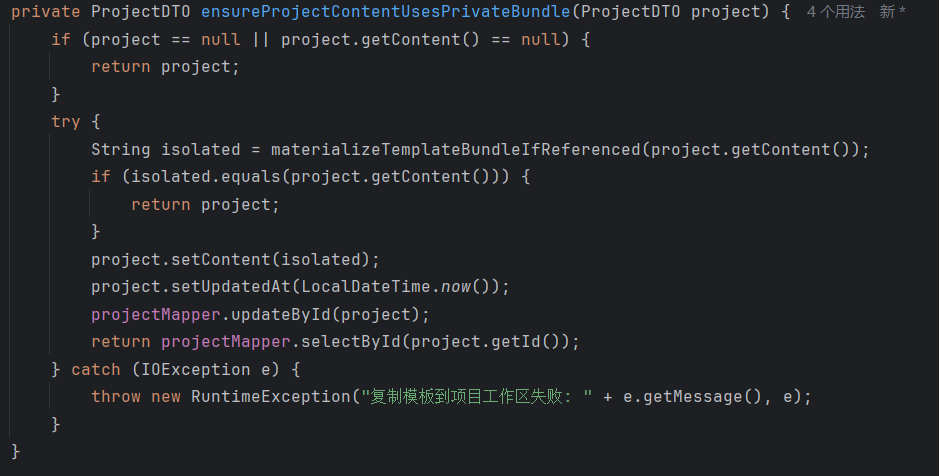
\includegraphics[width=0.75\linewidth]{project_41_e9d880e5.png}
    \caption{论文编译代码片段}
    \label{fig:placeholder}
\end{figure}

传统 LaTeX 编译通常依赖本地环境。用户需要先安装 TeX Live 或 MiKTeX，再使用本地编辑器或命令行执行编译命令。对于中文毕业论文，还需要注意编译引擎是否支持中文字体。如果用户选择了不合适的编译引擎，可能会出现中文乱码、字体缺失或编译失败等问题。编译成功后，用户还需要切换到 PDF 阅读器查看结果，修改后再重新编译，整个过程需要在多个工具之间反复切换。

本系统将源码编辑、编译引擎选择和 PDF 预览集成到同一编辑器页面。用户修改论文内容后，可以直接在工具栏选择编译引擎并点击编译。后端完成编译后，前端右侧预览区域自动刷新生成的 PDF 文件。这样用户可以在同一页面完成“编辑—编译—预览—修改”的循环过程。

\begin{table}[!ht]
    \centering
    \caption{在线编译预览案例运行过程}
    \label{tab:compile-preview-case}
    \begin{tabular}{|c|p{5cm}|p{6cm}|}
        \hline
        步骤 & 操作内容 & 运行结果 \\
        \hline
        1 & 用户进入论文编辑器页面 & 系统加载项目 LaTeX 源码和 PDF 预览区域 \\
        \hline
        2 & 用户修改章节内容或插入组件 & 编辑器中的源码实时更新 \\
        \hline
        3 & 用户选择 xelatex 编译引擎 & 系统记录本次编译使用的引擎类型 \\
        \hline
        4 & 用户点击编译按钮 & 后端创建编译目录并调用 LaTeX 编译命令 \\
        \hline
        5 & 编译成功后返回 PDF 路径 & 前端在预览区域显示最新 PDF 结果 \\
        \hline
    \end{tabular}
\end{table}

在线编译预览功能与传统本地编译方式的对比如表 \ref{tab:compile-compare} 所示。

\begin{table}[!ht]
    \centering
    \caption{在线编译预览与传统本地编译方式对比}
    \label{tab:compile-compare}
    \begin{tabular}{|c|p{5cm}|p{5cm}|}
        \hline
        对比项 & 传统本地 LaTeX 编译方式 & 本系统在线编译预览方式 \\
        \hline
        编译环境 & 用户需要自行安装和配置 TeX 环境 & 编译环境由服务器统一配置 \\
        \hline
        编译操作 & 需要使用本地编辑器或命令行编译 & 在浏览器中点击按钮即可编译 \\
        \hline
        引擎选择 & 用户需要了解不同引擎的适用场景 & 系统提供 pdflatex、xelatex、lualatex 选项 \\
        \hline
        结果查看 & 需要切换到 PDF 阅读器查看结果 & 编译后可在页面中直接预览 PDF \\
        \hline
        修改流程 & 编辑、编译、查看分散在不同工具中 & 编辑、编译、预览集中在同一页面中 \\
        \hline
    \end{tabular}
\end{table}

通过该案例可以看出，在线编译预览功能提高了论文排版流程的连贯性。用户不需要在本地安装复杂的 LaTeX 编译环境，也不需要频繁切换编辑器和 PDF 阅读器。对于本科毕业论文写作而言，这种方式能够减少环境配置和工具切换带来的干扰，使用户更加专注于论文内容修改和格式调整。

\section{文件导出模块的设计与实现}
文件导出模块用于满足用户在不同场景下的论文提交和编辑需求。系统主要支持 PDF、LaTeX 和 Word 三种格式导出。由于不同文档格式在结构表示和排版信息保留方面存在差异，文件转换过程中需要考虑内容结构识别与格式兼容问题\cite{dejean2006pdfxml}。

PDF 导出依赖 LaTeX 编译结果。当论文编译成功后，系统将生成的 PDF 文件保存到指定目录，并提供下载地址。用户点击导出 PDF 时，前端直接请求后端下载接口即可。

LaTeX 导出用于导出项目源码。系统根据项目 ID 查询当前项目的 latex\_content 字段，并生成 .tex 文件返回给用户。该功能适合用户后续在本地或其他 LaTeX 平台继续编辑。

Word 导出则通过文档转换工具实现。后端可以将 LaTeX 源码或编译生成的中间文件交由 Pandoc 转换为 .docx 文件。转换完成后，系统记录文件路径，并向前端返回下载链接。由于 LaTeX 与 Word 的排版机制不同，复杂模板、特殊宏包和部分公式环境在转换过程中可能存在兼容性问题，因此 Word 导出主要满足基础内容转换需求\cite{krewinkel2017pandoc}。

\begin{figure}[!ht]
    \centering
    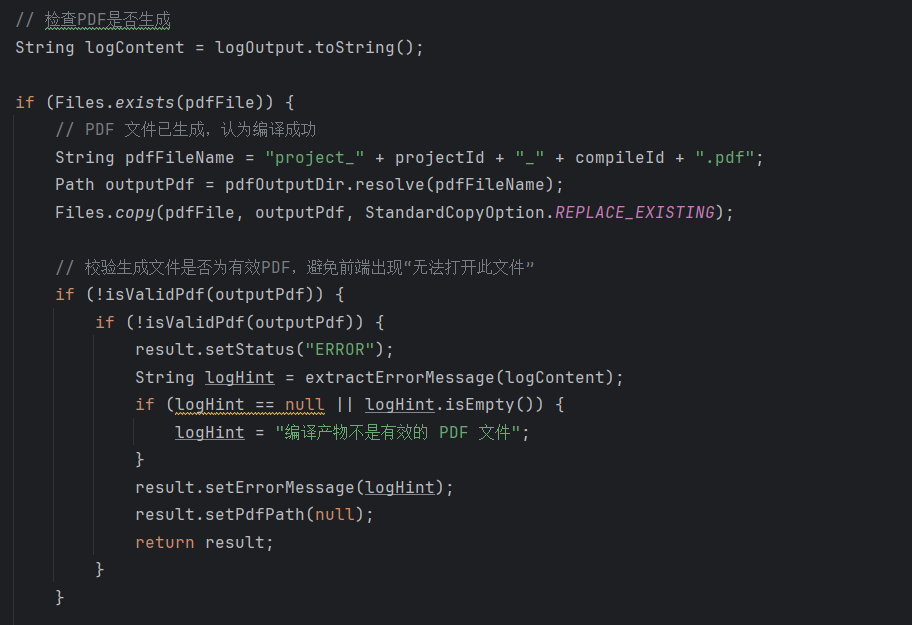
\includegraphics[width=0.75\linewidth]{project_41_e9286287.png}
    \caption{pdf下载代码片段}
    \label{fig:placeholder}
\end{figure}

\section{AI 辅助模块的设计与实现}
AI 辅助模块主要包括 AI 对话和编译错误分析两个功能。该模块的目标是降低用户使用 LaTeX 的难度，帮助用户理解排版命令、模板问题和编译错误。

AI 对话功能位于编辑器页面的上方工具栏。用户可以输入问题，例如“如何插入图片”“如何写数学公式”“为什么 xelatex 编译失败”等。前端将用户问题提交给后端，后端封装请求并调用 AI 接口。AI 返回结果后，前端以对话形式展示给用户。

编译错误分析功能与论文编译模块联动。当编译失败时，系统会保存错误日志。用户点击“AI 分析错误”按钮后，后端读取最近一次编译日志，并结合部分 LaTeX 源码构造提示词，请求 AI 分析错误原因。AI 返回内容通常包括错误原因、可能位置和修改建议\cite{gupta2017deepfix}。前端将分析结果展示在 AI 面板中，方便用户根据建议修改源码。

\begin{figure}[!ht]
    \centering
    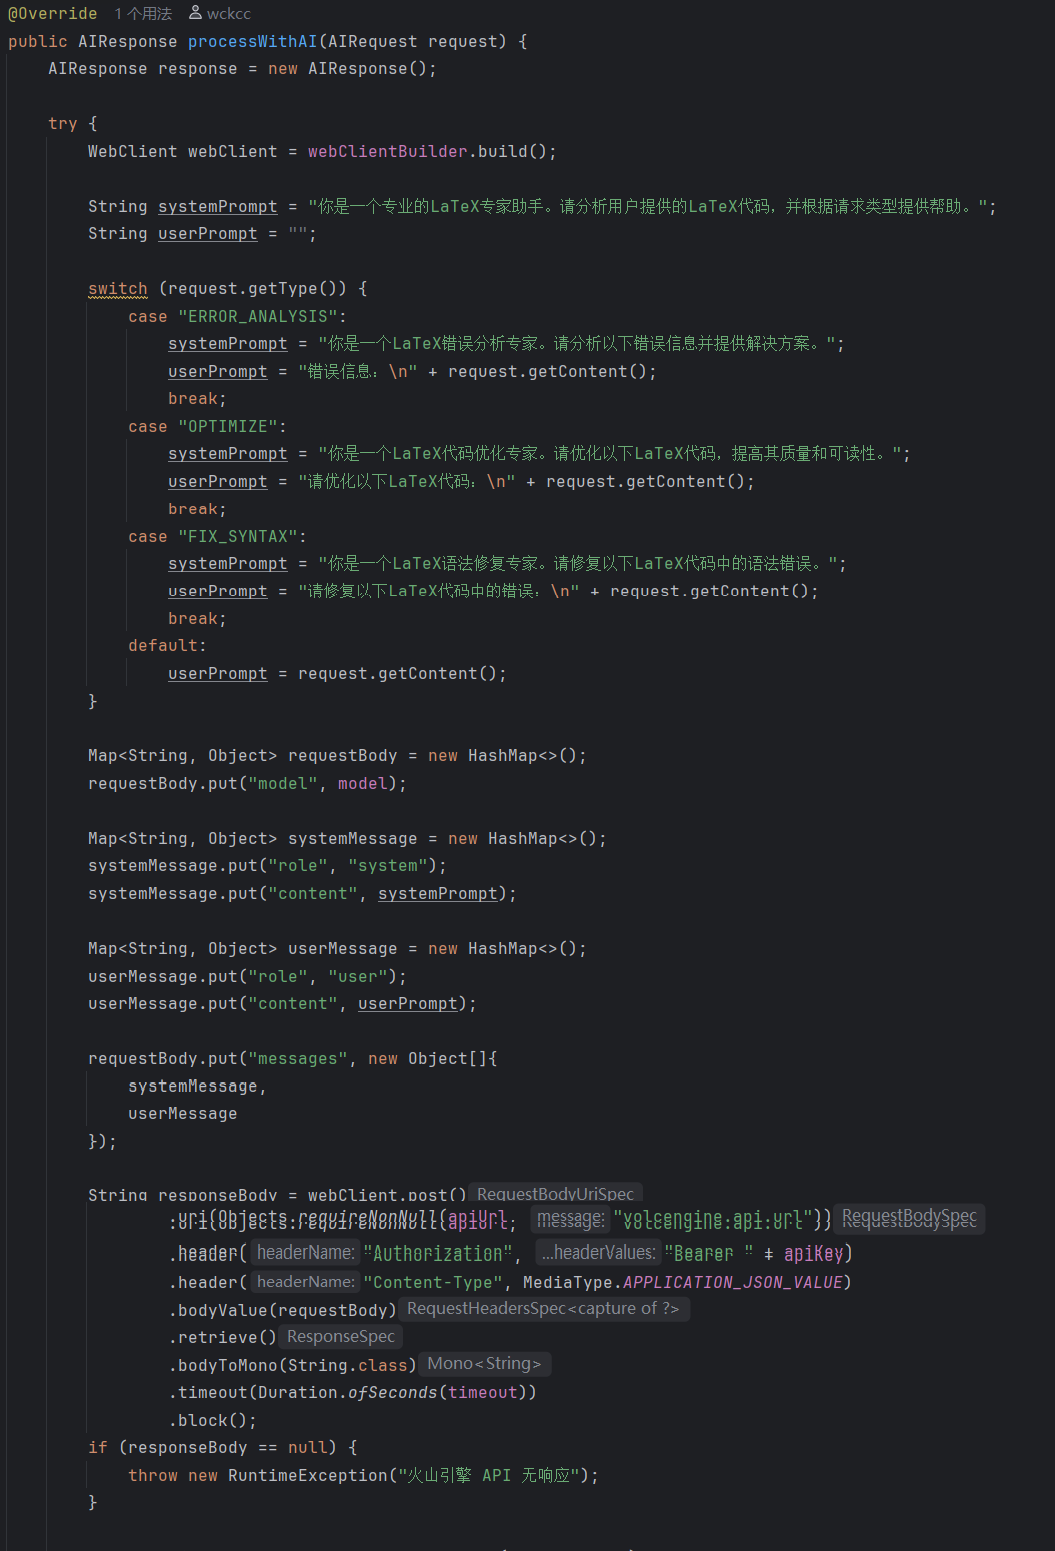
\includegraphics[width=0.75\linewidth]{project_41_c05eea7a.png}
    \caption{AI对话代码片段}
    \label{fig:placeholder}
\end{figure}

\section{核心功能测试}

为了验证系统主要功能是否能够正常运行，并考察系统在实际使用过程中的运行效果，本节对系统核心功能和基本性能进行了测试。测试内容包括用户登录、项目创建、LaTeX 编辑保存、论文编译、模板导入、文件导出和 AI 错误分析等功能，同时适当测试系统响应时间和内存占用情况。通过测试，可以判断系统是否满足前文需求分析中提出的功能要求和性能要求。

\subsection{测试环境}

系统测试在本地开发环境下进行。测试过程中，前端通过浏览器访问系统页面，后端服务运行在本地服务器环境中，数据库采用 MySQL 保存用户、项目、模板、编译记录和 AI 日志等数据。具体测试环境如表 \ref{tab:test-environment} 所示。

\begin{table}[!ht]
    \centering
    \caption{系统测试环境}
    \label{tab:test-environment}
    \begin{tabular}{|c|c|}
        \hline
        测试项 & 测试环境 \\
        \hline
        操作系统 & Windows 11 \\
        \hline
        浏览器 & Chrome / Edge \\
        \hline
        前端环境 & Vue 3、Vite \\
        \hline
        后端环境 & JDK 21、Spring Boot 3 \\
        \hline
        数据库 & MySQL \\
        \hline
        LaTeX 环境 & TeX Live，主要使用 XeLaTeX 编译 \\
        \hline
        测试工具 & 浏览器开发者工具、Postman、系统任务管理器 \\
        \hline
    \end{tabular}
\end{table}

\subsection{功能测试}

功能测试主要用于验证系统各模块是否能够按照预期完成操作。根据系统功能设计，本文选取用户登录、邮箱验证码、项目创建、论文保存、模板创建、LaTeX 编译、错误反馈、AI 错误分析和文件导出等典型操作进行测试。测试结果如表 \ref{tab:function-test} 所示。

\begin{table}[!ht]
    \centering
    \caption{核心功能测试表}
    \label{tab:function-test}
    \begin{tabular}{|c|c|p{6cm}|p{4cm}|}
        \hline
        测试编号 & 测试功能 & 测试内容 & 预期结果 \\
        \hline
        T1 & 用户登录 & 输入正确账号和密码 & 登录成功并进入项目列表 \\
        \hline
        T2 & 邮箱验证码 & 输入邮箱并发送验证码 & 邮箱收到验证码 \\
        \hline
        T3 & 创建项目 & 创建空白论文项目 & 项目创建成功并显示在列表中 \\
        \hline
        T4 & 保存论文 & 修改 LaTeX 内容并保存 & 数据库中项目内容更新 \\
        \hline
        T5 & 模板创建 & 选择模板创建项目 & 项目载入模板初始内容 \\
        \hline
        T6 & LaTeX 编译 & 使用 XeLaTeX 编译论文 & 成功生成 PDF 文件 \\
        \hline
        T7 & 编译失败反馈 & 输入错误 LaTeX 语法后编译 & 系统返回错误日志 \\
        \hline
        T8 & AI 错误分析 & 对错误日志进行 AI 分析 & 返回错误原因和修改建议 \\
        \hline
        T9 & PDF 导出 & 下载编译生成的 PDF 文件 & 成功下载 PDF 文件 \\
        \hline
        T10 & Word 导出 & 导出 docx 文件 & 成功生成 Word 文件 \\
        \hline
    \end{tabular}
\end{table}

从功能测试结果可以看出，系统能够完成用户登录、项目管理、在线编辑、模板载入、论文编译、文件导出和 AI 错误分析等主要功能。对于编译失败的情况，系统能够返回错误日志，并通过 AI 辅助功能给出相应的错误原因和修改建议，基本满足系统设计目标。

\subsection{性能测试}

除功能正确性外，系统运行性能也会影响用户的实际使用体验。由于本系统需要频繁进行项目保存、模板加载、LaTeX 编译、PDF 预览和 AI 错误分析等操作，因此本文选取接口响应时间、LaTeX 编译耗时和内存占用情况作为性能测试指标。

（1）接口响应时间测试。接口响应时间主要用于观察系统在常见业务操作下的处理速度。测试过程中，通过浏览器开发者工具和 Postman 记录用户登录、项目列表查询、论文保存、模板列表查询和编译日志查询等接口的响应时间。测试结果如表 \ref{tab:response-time-test} 所示。

\begin{table}[!ht]
    \centering
    \caption{接口响应时间测试结果}
    \label{tab:response-time-test}
    \begin{tabular}{|c|c|c|c|}
        \hline
        测试编号 & 测试内容 & 平均响应时间/ms & 测试结果 \\
        \hline
        P1 & 用户登录 & 79 & 正常 \\
        \hline
        P2 & 查询项目列表 & 3 & 正常 \\
        \hline
        P3 & 保存论文项目内容 & 3 & 正常 \\
        \hline
        P4 & 查询模板列表 & 4 & 正常 \\
        \hline
        P5 & 获取编译日志 & 3 & 正常 \\
        \hline
        P6 & AI 错误分析请求 & 37370 & 正常 \\
        \hline
    \end{tabular}
\end{table}

由表 \ref{tab:response-time-test} 可以看出，系统普通业务接口的响应时间基本保持在较短范围内，能够满足用户日常编辑和项目管理需求。AI 错误分析接口由于需要调用外部 AI 服务，响应时间明显高于普通业务接口，但仍处于可接受范围内。

（2）内存占用测试。内存占用测试主要用于观察系统在不同运行场景下的资源使用情况。测试过程中分别记录系统启动后、用户正常访问、执行 LaTeX 编译和调用 AI 分析时后端服务的内存占用情况，测试结果如表 \ref{tab:memory-test} 所示。

\begin{table}[!ht]
    \centering
    \caption{系统内存占用测试结果}
    \label{tab:memory-test}
    \begin{tabular}{|c|c|c|}
        \hline
        测试场景 & 内存占用情况/MB & 运行状态 \\
        \hline
        系统启动完成后 & 273 & 正常 \\
        \hline
        用户登录并浏览项目列表 & 273 & 正常 \\
        \hline
        编辑并保存论文内容 & 273 & 正常 \\
        \hline
        执行 LaTeX 编译 & 273 & 正常 \\
        \hline
        调用 AI 错误分析 & 274 & 正常 \\
        \hline
    \end{tabular}
\end{table}

由表 \ref{tab:memory-test} 可知，系统在普通页面访问和数据库操作场景下内存占用较为稳定。当执行 LaTeX 编译或调用 AI 分析功能时，内存占用会有所上升，这是因为系统需要临时处理 LaTeX 源文件、编译日志、生成文件以及 AI 请求数据。测试过程中未出现后端服务异常退出、页面长时间无响应或内存持续增长等问题，说明系统在当前测试规模下具有较好的运行稳定性。

\subsection{测试结果分析}

综合功能测试和性能测试结果可以看出，本文设计并实现的学术论文智能排版系统基本达到了预期目标。系统能够支持用户完成论文项目创建、LaTeX 在线编辑、模板加载、编译预览、文件导出和 AI 错误分析等核心操作。在性能方面，用户登录、项目查询、论文保存等普通业务接口响应时间较短，能够满足日常使用需求；系统内存占用整体稳定，没有出现明显资源泄漏或服务异常中断问题。

同时，测试结果也说明系统仍有进一步优化空间。首先，LaTeX 编译过程相比普通接口耗时较长，后续可以通过异步编译、编译任务队列和编译结果缓存等方式提升用户体验。其次，AI 错误分析功能依赖外部模型接口，响应时间受网络环境和模型服务状态影响较大，后续可以增加请求超时处理、错误重试机制和分析结果缓存机制。最后，在多用户同时编辑和编译的场景下，系统还需要进一步进行并发压力测试，以验证系统在更高访问量下的稳定性。

\section{本章小结}
本章对基于 JavaWeb 和 LaTeX 的学术论文智能排版系统进行了详细设计与实现说明。首先介绍了系统开发环境，然后分别对用户管理、论文项目管理、模板管理、LaTeX 在线编辑、论文编译与预览、文件导出和 AI 辅助等核心模块进行了详细阐述，说明了各模块的主要功能、实现流程和关键设计。最后，对系统核心功能进行了测试，验证了系统主要模块能够正常运行。本章内容为后续系统测试和总结分析提供了基础。

\chapter{总结与展望}

\section{总结}
本文围绕《基于JavaWeb和LaTeX的学术论文智能排版系统设计与实现》这一课题，设计并实现了一个面向学术论文写作场景的在线排版系统。系统针对传统论文排版过程中格式调整复杂、LaTeX学习成本较高、模板使用不便以及编译错误难以理解等问题，将论文项目管理、模板管理、LaTeX在线编辑、论文编译、PDF预览、文件导出和AI辅助等功能整合到统一平台中，为用户提供了较为完整的论文写作与排版流程。

在系统设计方面，本文采用前后端分离架构。前端基于Vue 3和Vite实现页面展示与用户交互，后端基于Spring Boot、MyBatis和MySQL实现业务逻辑处理与数据持久化。系统通过接口完成前后端数据交互，并结合token机制实现用户身份认证和权限控制，保证用户能够安全地管理自己的论文项目。

在功能实现方面，系统完成了用户注册登录、邮箱验证码、个人资料管理、论文项目创建与保存、模板载入、管理员zip模板导入、LaTeX源码在线编辑、多引擎编译、PDF预览、Word/LaTeX/PDF导出、AI对话辅助和编译错误分析等功能。其中，LaTeX在线编辑与论文编译是系统的核心功能，用户可以通过浏览器完成论文源码编辑，并使用pdflatex、xelatex、lualatex等编译引擎生成PDF文件。

此外，系统针对LaTeX模板依赖文件较多的问题，在模板导入和编译过程中尽量保留模板目录结构，减少因.cls、.sty、.bib等文件缺失造成的编译失败。同时，系统引入AI辅助功能，在用户遇到LaTeX语法问题或编译错误时，能够提供一定的解释和修改建议，提高了系统的易用性。
通过开发与测试，系统基本实现了预期功能，能够满足用户进行论文在线编辑、模板使用、编译预览和文件导出的基本需求，具有一定的实用价值。

\section{展望}
虽然本系统已经完成了主要功能，但仍存在一些不足，需要在后续继续完善。

首先，系统的模板库仍需扩充。目前系统支持模板导入和载入，但模板数量有限，后续可以增加更多高校毕业论文模板、期刊论文模板和会议论文模板，并为模板提供编译说明和预览效果。

其次，复杂LaTeX模板的兼容性仍有提升空间。部分模板可能依赖特殊宏包、字体文件或多轮编译流程，后续可以增加模板自动检测功能，根据模板内容自动推荐合适的编译引擎和编译方式。

再次，AI辅助功能还可以进一步优化。后续可以结合错误行号、源码上下文和编译日志，提高AI错误分析的准确性，也可以增加LaTeX代码补全、格式检查和自动修改建议等功能。

最后，系统在协作编辑和安全性方面还可以继续增强。后续可以支持多人协同编辑、历史版本管理和导师批注功能；同时加强文件上传校验、编译任务隔离和接口访问控制，提高系统稳定性和安全性。

综上所述，基于JavaWeb和LaTeX的学术论文智能排版系统具有一定应用前景。随着模板库、AI辅助能力、协同编辑能力和安全机制的不断完善，系统能够为用户提供更加便捷、高效的论文写作与排版支持。

\end{document}